\documentclass[11pt]{article}
\usepackage[margin=0.88in]{geometry}
\usepackage{amsmath,amssymb,amsfonts,amsthm,mathtools}
\usepackage{booktabs,longtable,array,multirow}
\usepackage{enumitem}
\usepackage{xcolor}
\usepackage{hyperref}
\usepackage{tikz}
\usetikzlibrary{arrows.meta,positioning,fit,calc,shapes.geometric,decorations.pathmorphing}
\usepackage{listings}
\usepackage{microtype}
\usepackage{caption}
\usepackage{graphicx}
\usepackage{subcaption}
\usepackage{float}
\usepackage{needspace}
\usepackage{mathrsfs}
\definecolor{darkblue}{RGB}{25,74,126}
\definecolor{darkgreen}{RGB}{20,112,80}
\definecolor{darkred}{RGB}{143,45,45}
\definecolor{softgray}{RGB}{245,247,250}
\definecolor{softblue}{RGB}{237,246,255}
\definecolor{softgreen}{RGB}{237,250,244}
\definecolor{softorange}{RGB}{255,247,236}
\definecolor{softpurple}{RGB}{246,241,252}
\hypersetup{colorlinks=true, linkcolor=darkblue, citecolor=darkgreen, urlcolor=darkblue}
\lstset{basicstyle=\ttfamily\small,breaklines=true,columns=fullflexible,frame=single,backgroundcolor=\color{softgray}}
\setlist[itemize]{leftmargin=*,itemsep=2pt,topsep=2pt}
\setlist[enumerate]{leftmargin=*,itemsep=2pt,topsep=2pt}
\sloppy

\newtheorem{theorem}{Theorem}[section]
\newtheorem{proposition}[theorem]{Proposition}
\newtheorem{lemma}[theorem]{Lemma}
\newtheorem{corollary}[theorem]{Corollary}
\newtheorem{definition}[theorem]{Definition}
\newtheorem{example}[theorem]{Example}
\newtheorem{remark}[theorem]{Remark}

\newcommand{\RR}{\mathbb{R}}
\newcommand{\ZZ}{\mathbb{Z}}
\newcommand{\NN}{\mathbb{N}}
\newcommand{\QQ}{\mathbb{Q}}
\newcommand{\CC}{\mathbb{C}}
\newcommand{\FF}{\mathbb{F}}
\newcommand{\calX}{\mathcal{X}}
\newcommand{\calK}{\mathcal{K}}
\newcommand{\calM}{\mathcal{M}}
\newcommand{\calD}{\mathcal{D}}
\newcommand{\calF}{\mathcal{F}}
\newcommand{\calG}{\mathcal{G}}
\newcommand{\calC}{\mathcal{C}}
\newcommand{\calU}{\mathcal{U}}
\newcommand{\calI}{\mathcal{I}}
\newcommand{\calR}{\mathcal{R}}
\newcommand{\calL}{\mathcal{L}}
\newcommand{\calQ}{\mathcal{Q}}
\newcommand{\calP}{\mathcal{P}}
\newcommand{\calH}{\mathcal{H}}
\newcommand{\calV}{\mathcal{V}}
\newcommand{\OO}{\mathcal{O}}
\newcommand{\Spec}{\operatorname{Spec}}
\newcommand{\Proj}{\operatorname{Proj}}
\newcommand{\Hom}{\operatorname{Hom}}
\newcommand{\Ext}{\operatorname{Ext}}
\newcommand{\Tor}{\operatorname{Tor}}
\newcommand{\rank}{\operatorname{rank}}
\newcommand{\dist}{\operatorname{dist}}
\newcommand{\diag}{\operatorname{diag}}
\newcommand{\softmax}{\operatorname{softmax}}
\newcommand{\CE}{\operatorname{CE}}
\newcommand{\argmax}{\operatorname*{arg\,max}}
\newcommand{\bitsperbyte}{\mathrm{bits\mbox{-}per\mbox{-}byte}}
\newcommand{\loss}{\mathcal{L}}
\newcommand{\eps}{\varepsilon}
\newcommand{\onecone}{one-dimensional cone}
\newcommand{\calA}{\mathcal{A}}
\newcommand{\calB}{\mathcal{B}}
\newcommand{\calE}{\mathcal{E}}
\newcommand{\calJ}{\mathcal{J}}
\newcommand{\calN}{\mathcal{N}}
\newcommand{\calO}{\mathcal{O}}
\newcommand{\calS}{\mathcal{S}}
\newcommand{\calT}{\mathcal{T}}
\newcommand{\calW}{\mathcal{W}}
\newcommand{\calY}{\mathcal{Y}}
\newcommand{\calZ}{\mathcal{Z}}
\newcommand{\onecones}{one-dimensional cones}
\numberwithin{equation}{section}

\begin{document}
\begin{titlepage}
\centering
{\Huge\bfseries ToricGT III:\par}
\vspace{4pt}
{\Huge\bfseries Sheafified MCP Memory, Graph-Structured Vector Retrieval, and Long-Context Tropical Ring Attention\par}
\vspace{10pt}
{\Large A NeurIPS-style third-iteration research article for model context protocols, markdown memory, knowledge graphs, 1--10M-token context windows, and bits-per-byte-safe reasoning agents\par}
\vspace{18pt}
{\large Amelie Schreiber}\par
{\large June 2026}\par
\vfill
\begin{abstract}
ToricGT I made toric geometry operational for graph-token reasoning by attaching finite BGG, Koszul, Gale-dual, and toric-chart certificates to hidden trajectories. ToricGT II replaced isolated certificates by a dynamical theory: a reasoning step became a standardized packet whose filtered simplicial complexes, multigraded persistence modules, sheaves, vector bundles, derived objects, and toric chart codes evolve under a learned graph-to-graph map. This paper develops ToricGT III. The object of study is no longer only a reasoning trajectory inside the model, but the external context substrate through which modern agents operate: model context protocols (MCPs), markdown-style memory, tool/resource/prompt traces, and knowledge graphs vectorized into embeddings with adjacency and provenance.

We define an MCP-memory object as a typed graph of messages, resources, tools, prompts, markdown blocks, knowledge-graph entities, schema fields, permissions, and update events. From it we build an efficient graph-structured vector database: every node, edge, simplex, sheaf section, Cox coordinate, and certificate summary receives a vector, a quantized code, adjacency links, and provenance metadata. A learned projection head maps the full database into a small retrieval space for approximate nearest-neighbor search, while graph expansion, sheaf gluing, toric quantization, and derived persistence rerank the candidates. The new long-context contribution is to treat the iterative reasoning context window itself as a finite but very large toric dynamical object: a 1--10M-token canvas that is progressively filled by reasoning blocks, MCP observations, markdown memories, knowledge-graph neighborhoods, verifier traces, and behavior-control sections until the required answer length $L_C\le 10^7$ is reached. Tropical ring attention gives an exact max-plus streaming semantics for active evidence and provenance over the full context, while projected graph retrieval supplies a sublinear candidate generator. We prove stability, finite-generation, projection-preservation, quantization-error, tropical-ring exactness, stopping-time, sheaf-gluing, derived mapping-cone, and ergodic-average theorems that explain when such a system improves reasoning quality, retrieval accuracy, behavior control, and held-out bits-per-byte. Finally, we give a 40-objective training catalogue plus a long-context extension catalogue for 1--10M-token MCP/memory/KG reasoning.
\end{abstract}
\vfill
\begin{minipage}{0.92\textwidth}
\textbf{Design contract.} Toric geometry is used as a compression, retrieval, and control instrument. Cones, \onecones, affine semigroups, normal fans, Cox coordinates, sheaves, vector bundles, differential forms, Cech complexes, local cohomology, Stanley-Reisner rings, derived categories, tableaux, root-system combinatorics, and ergodic theory enter only through finite certificates, compact vector codes, low-rank probes, and auditable retrieval traces. Any structure that improves the teacher but harms quantized held-out bits-per-byte remains teacher-side.  The 1--10M-token context window is governed by the same rule: the agent fills context only while marginal retrieved or generated slots improve net prediction, verification, or control.
\end{minipage}
\end{titlepage}
\tableofcontents
\clearpage

\section{Purpose, scope, and continuity with ToricGT I--II}
\subsection{Why a third paper is needed}
ToricGT I and II focus on the model's internal reasoning geometry. That is necessary but insufficient for agents that reason by calling tools, reading resources, editing memories, and traversing knowledge graphs. In such agents, the context system is not a passive prompt prefix. It is an evolving mathematical object. A tool call creates a typed edge; a resource response creates a provenance-bearing section; a markdown memory edit changes a local chart; a knowledge-graph expansion changes adjacency; a retrieved context package changes future token probabilities. If those operations are treated as flat text concatenation, the model wastes capacity relearning locality, provenance, schema compatibility, and behavior constraints from surface tokens. The ToricGT III thesis is that these structures should be stored, retrieved, trained, and compressed as graph-structured algebraic objects.

The immediate engineering target is a vector database whose records are not independent vectors. Each record is a node or cell in a typed graph; its vector is indexed together with adjacency, filtration, sheaf restrictions, quantized toric chart code, permissions, freshness, provenance, and known failure modes. The retrieval head sees a projected version of this database, not the full expensive object. The model uses fast approximate search first, then graph expansion and exact finite audits second. This is the same design pattern used in the earlier papers: train with rich finite structure; deploy only the compressed pieces that improve held-out bits-per-byte, verified reasoning, or behavior control.

\subsection{Summary of ToricGT I}
ToricGT I represents structured tasks as typed graphs, tokenizes node and edge objects equivariantly, and uses graph-token Transformer blocks with ordinary attention, tropical attention, noncommutative-torus phase channels, GraphCG concept coordinates, Soft-MoE routing, GFlowNet graph-of-thought search, and trajectory memory. Its toric BGG layer adds finite certificates: sign-vector posets, standard filtrations, sparse differentials, Betti profiles, Gale-dual labels, active faces of Newton polytopes, toric-ideal relations, Euler-Koszul probes, and homological consistency checks. The central deployment rule is conservative: the deployable model retains a probe only if ablations show validation bits-per-byte lift, reasoning-quality lift, retrieval improvement, or behavior reliability after artifact-byte accounting and quantized export.

ToricGT I is most naturally viewed as a theory of \emph{reasoning certificates}. It asks whether a hidden trajectory behaves like an exact finite algebraic object: a chain complex, a standard-object filtration, a toric module, a combinatorial resolution, or a behavior-corridor section. That framing already contains a memory component: trajectory retrieval should prefer helper paths with compatible BGG or resolution signatures, not merely nearby final embeddings.

\subsection{Summary of ToricGT II}
ToricGT II turns those certificates into a dynamical theory. A reasoning step is a padded packet
\begin{equation}
 x_t=(H_t, G_t, M_t, V_t, B_t, C_t, \tau_t),
\end{equation}
where $H_t$ is a hidden table, $G_t$ is a graph-of-thought neighborhood, $M_t$ is memory state, $V_t$ records verifier fields, $B_t$ records behavior-corridor coordinates, $C_t$ records finite certificates, and $\tau_t$ records a toric chart code. From $x_t$ one constructs filtered complexes $\calK_t$, multigraded persistence modules $\calM_t$, derived objects $\calD_t$, sheaf or vector-bundle charts $\calF_t$, and toric embedding codes. The learned map $T_\theta:x_t\mapsto x_{t+1}$ induces dynamics on all of them. ToricGT II then proves finite-generation and stability statements, uses mapping-cone residuals to measure failures of functoriality, and applies ergodic averages to long-run bits-per-byte, topology, verifier accuracy, and behavior-corridor cost.

The key principle carried into ToricGT III is the side-information identity. If a prefix-visible context certificate $Z_t$ helps predict the next byte $B_t$, then an optimal predictor can reduce expected log loss by
\begin{equation}
 I(B_t;Z_t\mid \mathcal{F}_t)
\end{equation}
bits, where $\mathcal{F}_t$ is the strict prefix sigma-field. If $Z_t$ is decorative, future-dependent, too expensive, or not robust after quantization, it should not be serialized into the deployed system.

\subsection{What ToricGT III adds}
ToricGT III moves the mathematical object from \emph{inside} a reasoning step to the context ecosystem around it. Its objects are MCP traces, markdown memories, graph-structured knowledge bases, vector indexes, retrieval heads, quantizers, and context-packing policies. The paper makes four contributions.

\begin{enumerate}
\item It defines a protocol-context graph category whose objects include MCP messages, tools, resources, prompts, results, markdown blocks, graph entities, edge relations, permissions, and provenance.
\item It turns markdown memory and knowledge graphs into sheaves, vector bundles, filtered complexes, and multigraded persistence modules, so that memory consistency and retrieval quality can be audited by finite algebra.
\item It constructs graph-structured vector databases with learned projections and quantized toric codes, and proves retrieval stability under projection and quantization margins.
\item It gives a trainable objective catalogue for improving bits-per-byte, reasoning quality, retrieval, accuracy, tone/personality control, safety boundaries, and artifact efficiency.
\end{enumerate}

\begin{figure}[H]
\centering
\resizebox{\textwidth}{!}{%
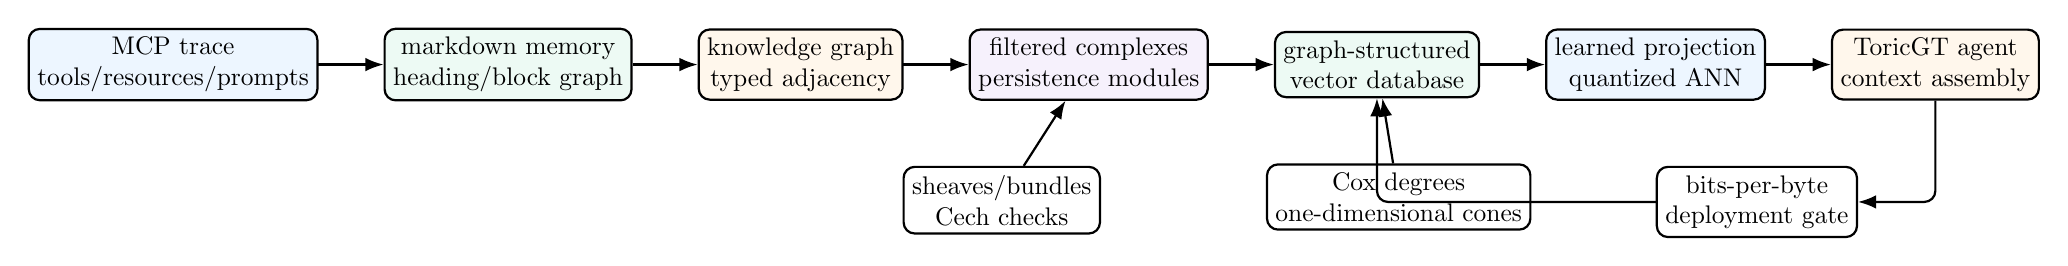
\begin{tikzpicture}[>=Latex,node distance=0.9cm,rounded corners,thick,scale=0.92, every node/.style={transform shape}]
\tikzstyle{box}=[draw,fill=softgray,minimum width=2.6cm,minimum height=0.82cm,align=center]
\tikzstyle{smallbox}=[draw,fill=white,minimum width=2.2cm,minimum height=0.62cm,align=center]
\node[box,fill=softblue] (mcp) {MCP trace\\tools/resources/prompts};
\node[box,fill=softgreen,right=of mcp] (mem) {markdown memory\\heading/block graph};
\node[box,fill=softorange,right=of mem] (kg) {knowledge graph\\typed adjacency};
\node[box,fill=softpurple,right=of kg] (complex) {filtered complexes\\persistence modules};
\node[box,fill=softgreen,right=of complex] (vdb) {graph-structured\\vector database};
\node[box,fill=softblue,right=of vdb] (proj) {learned projection\\quantized ANN};
\node[box,fill=softorange,right=of proj] (agent) {ToricGT agent\\context assembly};
\draw[->] (mcp) -- (mem);
\draw[->] (mem) -- (kg);
\draw[->] (kg) -- (complex);
\draw[->] (complex) -- (vdb);
\draw[->] (vdb) -- (proj);
\draw[->] (proj) -- (agent);
\node[smallbox,below=of complex,xshift=-1.2cm] (sheaf) {sheaves/bundles\\Cech checks};
\node[smallbox,below=of vdb,xshift=0.3cm] (toric) {Cox degrees\\\onecones};
\node[smallbox,below=of proj,xshift=1.4cm] (gate) {bits-per-byte\\deployment gate};
\draw[->] (sheaf) -- (complex);
\draw[->] (toric) -- (vdb);
\draw[->] (agent) |- (gate);
\draw[->] (gate) -| (vdb);
\end{tikzpicture}}
\caption{ToricGT III pipeline. MCP traces, markdown memory, and knowledge graphs are converted into filtered, sheafified, graph-structured vector databases. A learned projection enables efficient retrieval; toric and derived certificates audit the retrieved context before it affects the model.}
\end{figure}

\section{MCPs as typed protocol graphs}
\subsection{Protocol primitives}
The current MCP specification describes an open protocol for integrating LLM applications with external data sources and tools. It uses JSON-RPC 2.0 communication among hosts, clients, and servers; servers can expose resources, prompts, and tools, while clients can expose features such as sampling, roots, and elicitation. The tool feature is model-controlled: servers expose named tools with schemas, clients list tools, and tool calls return structured or unstructured content with error and security handling. ToricGT III abstracts these details into a finite typed graph so they can be embedded, indexed, audited, and trained.

\begin{definition}[Protocol event alphabet]
Let $\mathsf{T}$ be a finite set of event types:
\begin{equation}
\mathsf{T}=\{\mathsf{message},\mathsf{tool},\mathsf{toolcall},\mathsf{toolresult},\mathsf{resource},\mathsf{prompt},\mathsf{schema},\mathsf{permission},\mathsf{memory},\mathsf{kg},\mathsf{verifier}\}.
\end{equation}
A protocol event is a tuple
\begin{equation}
 e=(\mathrm{id},\tau, t, \mathrm{payload},\mathrm{schema},\mathrm{principal},\mathrm{provenance},\mathrm{visibility}),
\end{equation}
where $\tau\in\mathsf{T}$, $t$ is logical time, $\mathrm{principal}$ records the user, agent, server, or subsystem, and $\mathrm{visibility}$ records whether the event is prefix-visible for scoring.
\end{definition}

\begin{definition}[MCP context graph]
An MCP context graph is a typed attributed directed multigraph
\begin{equation}
G_{\mathrm{mcp}}=(V,E,s,t,\tau_V,\tau_E,x,e,p,\pi),
\end{equation}
where vertices are protocol events, edges record temporal succession, call-return linkage, resource references, prompt instantiation, schema validation, permission flow, memory update, or knowledge-graph relation, $x_v$ and $e_a$ are bounded real and symbolic attributes, $p$ is provenance metadata, and $\pi$ is a prefix-visibility mask.
\end{definition}

This graph representation deliberately separates semantic content from protocol legality. A tool call may be semantically useful but fail a schema constraint; a resource may be relevant but not visible under the current permission boundary; a memory block may be accurate but stale. These distinctions become graph features rather than prompt comments.

\begin{proposition}[Finite traces give finite context graphs]
Every finite MCP interaction trace with finitely many messages, tool calls, resource references, prompts, and memory updates determines a finite MCP context graph. Relabeling internal event identifiers induces a graph isomorphism preserving types, temporal order, call-return edges, schemas, and provenance.
\end{proposition}
\begin{proof}
The trace contains finitely many protocol events, so the vertex set is finite. Each declared relation among events is binary and belongs to a finite edge-type set; hence the edge multiset is finite. Replacing event identifiers by a bijection carries every event and every relation endpoint to the corresponding event and endpoint. Since types, schemas, time order, and provenance are stored as attributes rather than names, they are preserved. Thus identifier relabeling is graph isomorphism.
\end{proof}

\subsection{Context records and prefix safety}
ToricGT III distinguishes three levels of context storage.
\begin{enumerate}
\item A \emph{raw event store} contains exact JSON, text, files, and tool results.
\item A \emph{structured graph store} contains typed vertices, edges, schemas, permissions, timestamps, and provenance.
\item A \emph{projected vector index} contains compact codes used for fast retrieval.
\end{enumerate}
The raw event store is authoritative for audit. The structured graph store is authoritative for legal and provenance constraints. The projected index is a speed layer and must be treated as lossy.

\begin{definition}[Prefix-safe retrieval feature]
Let $\mathcal{F}_t$ be the sigma-field generated by the interaction prefix before byte $b_t$ is scored. A retrieval feature $Z_t$ is prefix-safe if $Z_t$ is $\mathcal{F}_t$-measurable. A training or evaluation run is prefix-safe if every retrieval, cache, graph edge, quantized code, and certificate used to predict $b_t$ is prefix-safe.
\end{definition}

\begin{theorem}[Side-information limit for context retrieval]
Let $B_t$ be the next byte and let $Z_t$ be a prefix-safe retrieval certificate. Among all normalized predictors, the expected log-loss improvement from revealing $Z_t$ in addition to $\mathcal{F}_t$ is at most
\begin{equation}
 I(B_t;Z_t\mid \mathcal{F}_t)
\end{equation}
bits, with equality for the true conditional distributions.
\end{theorem}
\begin{proof}
The optimal predictor without $Z_t$ is $p(B_t\mid\mathcal{F}_t)$ and has expected base-two log loss $H(B_t\mid\mathcal{F}_t)$. The optimal predictor with $Z_t$ is $p(B_t\mid\mathcal{F}_t,Z_t)$ and has expected loss $H(B_t\mid\mathcal{F}_t,Z_t)$. The difference is the conditional mutual information by definition:
\begin{equation}
H(B_t\mid\mathcal{F}_t)-H(B_t\mid\mathcal{F}_t,Z_t)=I(B_t;Z_t\mid\mathcal{F}_t).
\end{equation}
Any other predictor has no lower expected log loss than the conditional distribution, by nonnegativity of conditional KL divergence.
\end{proof}

This theorem is the compression discipline for the whole paper. A clever algebraic retrieval code is valuable only if it is prefix-visible and has conditional information about future bytes, verified answers, or behavior decisions. Otherwise it is a decorative source of latency and artifact bytes.

\section{Markdown memory and knowledge graphs}
\subsection{Markdown memory as a block poset}
Markdown memory has a useful latent geometry. Headings define a rooted block tree; links define cross-edges; bullets and tables define local product structure; code blocks define typed resources; front matter defines metadata. Treating a markdown file as flat text discards that geometry.

\begin{definition}[Markdown block graph]
A markdown memory document $D$ is parsed into a block graph
\begin{equation}
G_D=(V_D,E_D),
\end{equation}
where vertices are headings, paragraphs, bullets, table rows, code blocks, links, citations, and front-matter fields. There is a containment edge $u\to v$ when block $v$ is inside block $u$, an order edge when $v$ follows $u$ inside the same parent, and a reference edge when a link, citation, or identifier connects two blocks. Each vertex has text $c_v$, metadata $m_v$, embedding $z_v$, and permission/freshness fields.
\end{definition}

The block graph supports three important operations: restriction to a heading subtree, gluing of compatible local edits, and conflict detection across overlapping memories. These are sheaf operations.

\begin{definition}[Memory sheaf]
Let $P_D$ be the poset of markdown blocks ordered by containment, and give it the Alexandrov topology. A memory sheaf $\calF_D$ assigns to each block $v$ a vector space or finite set $\calF_D(v)$ of admissible local sections: summaries, embeddings, provenance tuples, evidence claims, tone constraints, or tool-result schemas. For $u\preceq v$ there is a restriction map
\begin{equation}
 \rho_{vu}:\calF_D(v)\to \calF_D(u).
\end{equation}
A global memory section is a compatible family $(s_v)$ such that $\rho_{vu}(s_v)=s_u$ whenever $u\preceq v$.
\end{definition}

\begin{example}[A pragmatic memory conflict]
Suppose a project memory file has sections ``dataset'', ``license'', and ``current experiment''. A retrieved tool result updates the dataset version. The license section restricts to a constraint ``noncommercial''. A generated answer that combines the new dataset version with an old commercial-use statement is a Cech-gluing failure: two local sections agree on some lexical keys but disagree on a restriction induced by the license field.
\end{example}

\begin{definition}[Cech memory residual]
Let $\calU=\{U_i\}$ be a finite cover of a memory block graph by heading neighborhoods or retrieval windows. If a model predicts local sections $s_i\in\calF(U_i)$, define
\begin{equation}
\loss_{\check C}(s)=\sum_{i<j}\|\rho_{i,ij}(s_i)-\rho_{j,ij}(s_j)\|^2_{W_{ij}}
+\lambda\sum_{i<j<k}\|\delta s_{ijk}\|^2.
\end{equation}
The second term penalizes higher-order inconsistencies on triple overlaps when available.
\end{definition}

\begin{proposition}[Zero residual glues local memory sections]
Assume $\calF$ is a sheaf of vector spaces on a finite cover $\calU$ and all restrictions are represented exactly. If $\loss_{\check C}(s)=0$ and the cover is closed under pairwise intersections, then the local sections $s_i$ glue to a unique section on $\bigcup_i U_i$.
\end{proposition}
\begin{proof}
The first term being zero says that $s_i$ and $s_j$ have equal restrictions on each overlap $U_i\cap U_j$. This is exactly the compatibility hypothesis in the sheaf gluing axiom. The sheaf axiom gives existence of a section $s$ on the union with $s|_{U_i}=s_i$. If $s'$ is another such section, then $s$ and $s'$ agree on every element of the cover, hence the locality axiom gives $s=s'$.
\end{proof}

\subsection{Knowledge graphs as typed quivers and path algebras}
A knowledge graph is naturally a typed directed multigraph. Let $G=(V,E)$ with relation type map $\tau_E:E\to\mathcal{R}$. A path $p=e_k\cdots e_1$ has type word $\tau(p)=\tau(e_k)\cdots\tau(e_1)$. The path algebra $\FF G$ is the vector space spanned by paths, with multiplication by concatenation when endpoints match and zero otherwise. This algebra encodes query composition and tool/resource chaining.

\begin{definition}[Vectorized knowledge graph with adjacency]
A vectorized knowledge graph is a tuple
\begin{equation}
\mathbb{K}=(G,Z,R,A,\Gamma),
\end{equation}
where $G=(V,E)$ is a typed directed multigraph, $Z\in\RR^{|V|\times d}$ are node embeddings, $R_{\tau}\in\RR^{d\times d}$ are relation operators, $A_\tau\in\{0,1\}^{|V|\times |V|}$ are typed adjacency matrices, and $\Gamma$ stores provenance, permissions, freshness, and schema constraints.
\end{definition}

A retrieval head should not only ask whether $z_q$ is close to $z_v$. It should ask whether $v$ lies in a graph neighborhood whose relations, schemas, and provenance make it usable for the current reasoning step.

\begin{definition}[Path-consistent retrieval score]
For a query representation $h_q$, a candidate node $v$, and a path set $\mathcal{P}(q,v)$ from seed nodes to $v$, define
\begin{equation}
S(q,v)=\langle P_q h_q,P_z z_v\rangle+\max_{p\in\mathcal{P}(q,v)}\sum_{e\in p}\omega_{\tau(e)}-\lambda_{\rm stale}\,a_v-\lambda_{\rm perm}\,\nu_v-\lambda_{\rm glue}\,r_v.
\end{equation}
Here $P_q,P_z$ are learned projections, $a_v$ is age or staleness, $\nu_v$ is permission risk, and $r_v$ is a Cech or schema-gluing residual.
\end{definition}

The score is intentionally decomposable. Its first term is fast vector search. The path term is graph expansion. The last terms enforce memory quality and trust.

\section{Filtered complexes and multigraded modules for context databases}
\subsection{From context graphs to complexes}
The vector database should expose more than nearest neighbors. A set of retrieved records has topology: multiple evidence nodes may jointly support a claim; a tool result may bridge two resources; a contradiction may appear as a forbidden coactivation; a style/tone constraint may be valid only with certain evidence and permission sections.

\begin{definition}[Context filtration]
Let $\mathbb{D}$ be a graph-structured context database with node vectors $z_v$, edge types, trust scores $t_v$, freshness scores $f_v$, permission scores $p_v$, and role labels $r_v$. For a multifiltration index
\begin{equation}
\alpha=(\rho,\theta_{\rm trust},\theta_{\rm fresh},\theta_{\rm perm},\theta_{\rm role})\in P,
\end{equation}
define a simplicial complex $\calK_\alpha(\mathbb{D})$ as follows. A vertex $v$ is included if it passes the scalar thresholds. A simplex $\{v_0,\ldots,v_k\}$ is included if all vertices are included, pairwise projected distances are at most $\rho$, and the induced typed subgraph belongs to an allowed motif set $\Omega$.
\end{definition}

Typical allowed motifs include: multiple resources supporting the same claim; tool-call/result/resource triples; markdown heading/child/link triples; knowledge-graph paths of bounded length; and behavior-corridor bundles containing evidence, verifier, tone, and answer-commitment nodes.

\begin{definition}[Context persistence module]
For a field $\FF$ and homological degree $p$, define
\begin{equation}
\calM_p(\mathbb{D})(\alpha)=H_p(\calK_\alpha(\mathbb{D});\FF).
\end{equation}
The structure maps are induced by inclusions when $\alpha\le \beta$. If $P=\NN^s$ or a finite grid in $\NN^s$, this is a multigraded persistence module over $S=\FF[u_1,\ldots,u_s]$ after extending past the grid boundary.
\end{definition}

\begin{theorem}[Finite context persistence modules are finitely generated]
Let $P=\prod_{i=1}^s\{0,\ldots,L_i\}$ be a finite grid and suppose the context database has $n$ valid records. Extend $\calM_p(\mathbb{D})$ constantly after the grid boundary. Then $\calM_p(\mathbb{D})$ is a finitely generated multigraded module over $S=\FF[u_1,
\ldots,u_s]$.
\end{theorem}
\begin{proof}
There are finitely many grid points. At each grid point the complex has at most $2^n$ simplices, hence finite-dimensional homology. Choose a finite basis for every homology vector space at every grid point and place these basis elements as homogeneous generators in their grid degrees. The polynomial variables $u_i$ propagate generators along coordinate directions. After the grid boundary, the module is constant, so no new generators are needed. Thus finitely many homogeneous generators suffice.
\end{proof}

\subsection{Derived context objects and update maps}
The free resolution of a multigraded context persistence module is a compact algebraic summary of retrieval structure.
\begin{definition}[Derived context object]
Let $\calM_p(\mathbb{D})$ be a finite-grid context persistence module. A derived context object is a finite free resolution
\begin{equation}
F_\bullet(\mathbb{D}):0\to F_r\to\cdots\to F_0\to\calM_p(\mathbb{D})\to 0
\end{equation}
viewed up to quasi-isomorphism in $D^b(\mathrm{gr}\text{-}S)$, enriched with role labels, Cox degrees, schema labels, permission levels, and provenance classes.
\end{definition}

An MCP interaction updates the database. A new tool result may add a record; a memory edit may replace a section; a schema migration may rewrite fields; a knowledge-graph import may add many edges. This is a graph-to-graph map
\begin{equation}
U_\theta:\mathbb{D}_t\longrightarrow \mathbb{D}_{t+1}.
\end{equation}
When $U_\theta$ is learned, we need to audit whether it induces valid maps on complexes and derived objects.

\begin{definition}[Context chain-map residual]
Let $C_\bullet(\calK_\alpha(\mathbb{D}_t))$ and $C_\bullet(\calK_{s(\alpha)}(\mathbb{D}_{t+1}))$ be chain complexes for matched filtration indices. A proposed transport $F_{p,\alpha}$ has residual
\begin{equation}
\operatorname{Res}_{\partial}(F)=\sum_{p,\alpha}\|\partial_{t+1}F_{p,\alpha}-F_{p-1,\alpha}\partial_t\|_F^2.
\end{equation}
\end{definition}

\begin{theorem}[Mapping cone measures memory-update failure]
Let $F_\bullet:C_\bullet\to D_\bullet$ be a degree-zero map between finite chain complexes. If $F_\bullet$ is a chain map, $\operatorname{Cone}(F)$ is a complex and fits into a distinguished triangle $C_\bullet\to D_\bullet\to\operatorname{Cone}(F)\to C_\bullet[1]$. If $F_\bullet$ is not a chain map, the obstruction to $\operatorname{Cone}(F)$ being a complex is exactly $\partial_DF-F\partial_C$.
\end{theorem}
\begin{proof}
The cone differential is $\delta(d,c)=(\partial_Dd+Fc,-\partial_Cc)$. Squaring gives
\begin{equation}
\delta^2(d,c)=(\partial_D^2d+\partial_DFc-F\partial_Cc,\partial_C^2c)=(\partial_DF-F\partial_C)c.
\end{equation}
Thus $\delta^2=0$ precisely when $F$ is a chain map. In that case the standard cone construction gives the distinguished triangle in the derived category. Otherwise the displayed commutator is the exact failure term.
\end{proof}

\section{Graph-structured vector databases}
\subsection{Database object}
A standard vector database stores vectors and metadata. ToricGT III stores vectors as a graph-indexed sheafified complex.

\begin{definition}[Graph-structured vector database]
A graph-structured vector database is a tuple
\begin{equation}
\mathbb{D}=(G,Z,Y,Q,A,\calK,\calF,\Xi,\Pi),
\end{equation}
where:
\begin{itemize}
\item $G=(V,E)$ is a finite typed attributed graph.
\item $Z:V\to\RR^d$ assigns a high-dimensional vector to each node.
\item $Y:E\to\RR^{d_e}$ assigns an edge vector or relation operator.
\item $Q:V\cup E\to\mathcal{C}$ assigns quantized codes.
\item $A$ is the collection of typed adjacency matrices.
\item $\calK$ is a family of filtered complexes built from $G,Z,Y,A$.
\item $\calF$ is a cellular or Cech sheaf storing local sections and restrictions.
\item $\Xi$ stores exact finite certificates: Betti profiles, Cech residuals, schema checks, path-algebra normal forms, toric codes, and permission proofs.
\item $\Pi$ stores prefix-safety, freshness, security, and provenance policies.
\end{itemize}
\end{definition}

\begin{figure}[H]
\centering
\resizebox{\textwidth}{!}{%
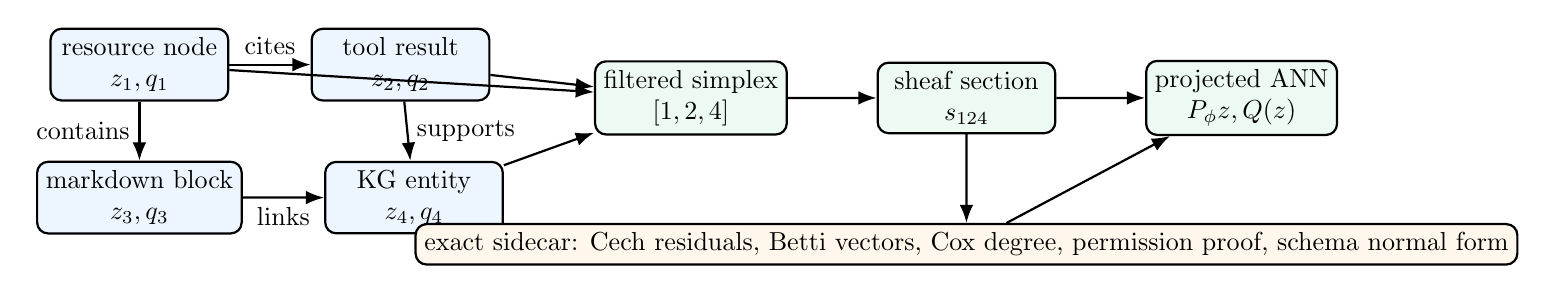
\begin{tikzpicture}[>=Latex,rounded corners,thick,node distance=0.8cm,scale=0.94,every node/.style={transform shape}]
\tikzstyle{nodebox}=[draw,fill=softblue,minimum width=2.4cm,minimum height=0.62cm,align=center]
\tikzstyle{cellbox}=[draw,fill=softgreen,minimum width=2.4cm,minimum height=0.62cm,align=center]
\node[nodebox] (n1) {resource node\\$z_1,q_1$};
\node[nodebox,right=1.1cm of n1] (n2) {tool result\\$z_2,q_2$};
\node[nodebox,below=0.8cm of n1] (n3) {markdown block\\$z_3,q_3$};
\node[nodebox,right=1.1cm of n3] (n4) {KG entity\\$z_4,q_4$};
\draw[->] (n1) -- node[above]{cites} (n2);
\draw[->] (n1) -- node[left]{contains} (n3);
\draw[->] (n3) -- node[below]{links} (n4);
\draw[->] (n2) -- node[right]{supports} (n4);
\node[cellbox,right=1.4cm of n2,yshift=-0.45cm] (simp) {filtered simplex\\$[1,2,4]$};
\draw[->] (n1) -- (simp);
\draw[->] (n2) -- (simp);
\draw[->] (n4) -- (simp);
\node[cellbox,right=1.2cm of simp] (sheaf) {sheaf section\\$s_{124}$};
\node[cellbox,right=1.2cm of sheaf] (ann) {projected ANN\\$P_\phi z, Q(z)$};
\draw[->] (simp) -- (sheaf);
\draw[->] (sheaf) -- (ann);
\node[draw,fill=softorange,below=1.2cm of sheaf,minimum width=6.4cm,align=center] (audit) {exact sidecar: Cech residuals, Betti vectors, Cox degree, permission proof, schema normal form};
\draw[->] (sheaf) -- (audit);
\draw[->] (audit) -- (ann);
\end{tikzpicture}}
\caption{Graph-structured vector database. Vectors are attached to protocol, memory, and knowledge-graph nodes, but retrieval also uses adjacency, simplices, sheaf sections, quantized codes, and exact sidecar certificates.}
\end{figure}

\subsection{Projected retrieval head}
The database may store high-dimensional vectors and expensive certificates, but the first retrieval stage must be small. Let $P_\phi:\RR^d\to\RR^r$ be a learned projection with $r\ll d$.

\begin{definition}[Projected graph retrieval]
Given a query packet $x$, produce a query vector $h_x$ and a projected query $\tilde h=P_q h_x$. For each database node $v$, store $\tilde z_v=P_z z_v$ and a quantized code $q_v$. The stage-one candidate set is
\begin{equation}
C_k(x)=\operatorname{TopK}_{v\in V}\;\langle \tilde h,\tilde z_v\rangle -\lambda_q\,d_Q(q_x,q_v),
\end{equation}
computed by an approximate nearest-neighbor index. The stage-two set is graph-expanded:
\begin{equation}
\overline C_k(x)=\{u:\operatorname{dist}_G(u,C_k(x))\le R,\;\Pi(u,x)=\mathrm{allow}\}.
\end{equation}
The final context set is obtained by reranking $\overline C_k(x)$ with sheaf, schema, provenance, and certificate scores.
\end{definition}

\begin{theorem}[Projection-margin retrieval preservation]
Let the exact retrieval score for a finite candidate set $C$ be $s_v$ and the projected score be $\tilde s_v$. Suppose the true best candidate $v^*$ has margin
\begin{equation}
\gamma=s_{v^*}-\max_{v\ne v^*}s_v>0.
\end{equation}
If $|s_v-\tilde s_v|\le\eps$ for every $v\in C$ and $\gamma>2\eps$, then the projected top-1 candidate equals the exact top-1 candidate.
\end{theorem}
\begin{proof}
For every $v\ne v^*$,
\begin{equation}
\tilde s_{v^*}-\tilde s_v\ge (s_{v^*}-\eps)-(s_v+\eps)=s_{v^*}-s_v-2\eps\ge\gamma-2\eps>0.
\end{equation}
Thus $v^*$ remains strictly highest-scoring under the projected scores.
\end{proof}

\begin{corollary}[Finite candidate Johnson-Lindenstrauss projection]
For a finite set of $N$ query and database vectors with bounded norm, a random projection to dimension $r=O(\eps^{-2}\log(N/\delta))$ preserves all pairwise inner products up to $\eps$ with probability at least $1-\delta$ after normalization. Therefore top-1 and top-$k$ retrieval are preserved whenever the exact score margins exceed the corresponding distortion bounds.
\end{corollary}
\begin{proof}
The Johnson-Lindenstrauss lemma preserves pairwise distances among the $N$ normalized vectors. Inner products are determined by squared distances through $\langle a,b\rangle=(\|a\|^2+\|b\|^2-\|a-b\|^2)/2$. Applying the previous theorem to the resulting inner-product distortion gives margin preservation.
\end{proof}

\subsection{Training the projection}
A learned projection can be trained with three simultaneous constraints: retrieval accuracy, metric preservation on hard pairs, and quantization compatibility.
\begin{align}
\loss_{\rm retr}&=-\log\frac{\sum_{v\in P(x)}\exp S_\phi(x,v)/\tau}{\sum_{v\in P(x)\cup N(x)}\exp S_\phi(x,v)/\tau},\\
\loss_{\rm dist}&=\mathbb E_{(u,v)\in\mathcal{H}}\left(\langle Pz_u,Pz_v\rangle-\langle z_u,z_v\rangle\right)^2,\\
\loss_{\rm qaware}&=\mathbb E_v\|Pz_v-\operatorname{deq}(Q(Pz_v))\|^2.
\end{align}
Here $P(x)$ are positive records, $N(x)$ hard negatives, $\mathcal{H}$ hard pairs near decision boundaries, and $Q$ is the quantizer. The final projection loss is
\begin{equation}
\loss_{\rm proj}=\loss_{\rm retr}+\lambda_d\loss_{\rm dist}+\lambda_q\loss_{\rm qaware}+\lambda_o\|P^\top P-I\|_F^2.
\end{equation}

\section{Toric quantization and Cox-coded context}
\subsection{Semigroup codes}
Quantization is not only a numerical compression technique. It is also a combinatorial algebraic object. Let $M\simeq\ZZ^m$ be a lattice of context codes. Choose code atoms $A=\{a_1,\ldots,a_s\}\subset M$, such as role, schema, source, tone, verifier state, trust band, and one-dimensional-cone chart identifiers. A record code is an element of the affine semigroup
\begin{equation}
S_A=\NN A=\left\{\sum_i n_i a_i:n_i\in\NN\right\}.
\end{equation}
The semigroup algebra $\CC[S_A]$ records multiplicative composition of context features. Relations among codes produce a toric ideal:
\begin{equation}
I_A=\langle x^u-x^v: Au=Av\rangle.
\end{equation}
A retrieval system should treat two code decompositions with the same semantic aggregate as equivalent unless provenance or permissions differ. Toric binomial losses enforce this equivalence.

\begin{definition}[Cox context code]
Let $\Sigma$ be a fan whose \onecones{} index context boundary types: evidence, verifier, memory, style, safety, schema, tool, resource, prompt, and answer commitment. A Cox context code is a monomial
\begin{equation}
 x^a=\prod_{\rho\in\Sigma(1)}x_\rho^{a_\rho}
\end{equation}
with multidegree $\deg(x^a)\in \operatorname{Cl}(X_\Sigma)$ or a learned finite quotient of that class group. Invalid coactivations are stored in an irrelevant or Stanley-Reisner ideal.
\end{definition}

\begin{theorem}[Quantized score perturbation bound]
Assume query and database vectors have norm at most $R$. Let $\hat z_v$ and $\hat h$ be quantized versions satisfying $\|z_v-\hat z_v\|\le\eta$ and $\|h-\hat h\|\le\eta$. Then
\begin{equation}
|\langle h,z_v\rangle-\langle \hat h,\hat z_v\rangle|\le 2R\eta+\eta^2.
\end{equation}
Therefore a ranking margin greater than $2(2R\eta+\eta^2)$ is stable under quantization.
\end{theorem}
\begin{proof}
Write
\begin{equation}
\langle h,z\rangle-\langle \hat h,\hat z\rangle=\langle h-\hat h,z\rangle+\langle \hat h,z-\hat z\rangle.
\end{equation}
Since $\|\hat h\|\le R+\eta$, the absolute value is bounded by $\eta R+(R+\eta)\eta=2R\eta+\eta^2$. The ranking statement follows by comparing the best candidate and any competitor, each of whose scores can shift by at most this amount.
\end{proof}

\begin{definition}[Toric quantization loss]
Let $c_v\in S_A$ be a discrete semigroup code and $\hat c_v$ a predicted code distribution. Let $\mathcal{B}$ be a set of low-degree toric binomial relations. Define
\begin{equation}
\loss_{\rm tq}=\mathrm{CE}(c_v,\hat c_v)+\lambda_{\rm bin}\sum_{x^u-x^v\in\mathcal{B}}\left\|\sum_i u_i\ell_i-\sum_i v_i\ell_i\right\|^2+\lambda_{\rm hole}\,\mathrm{Hole}(\hat c_v),
\end{equation}
where $\ell_i$ are logit coordinates and $\mathrm{Hole}$ penalizes predicted codes outside the saturated semigroup or normalized codebook.
\end{definition}

The practical benefit is compactness. Instead of storing long metadata strings for every record, the index stores small integer codes whose algebra is known. During retrieval, the model can combine codes by semigroup addition and reject invalid context packages by Stanley-Reisner nonface checks.

\section{Sheaves, vector bundles, and differential forms for retrieval control}
\subsection{Cellular sheaves over context graphs}
A cellular sheaf over a graph or simplicial complex attaches data to cells and restriction maps to incidences. In ToricGT III, a vertex section may be a local summary, an embedding, a permission token, a style state, or a schema object. An edge restriction describes how two records agree on a shared claim, entity, tool schema, or behavior corridor.

\begin{definition}[Context sheaf on a complex]
Let $K$ be a finite simplicial complex built from retrieved context records. A cellular context sheaf $\calF$ assigns a vector space $\calF(\sigma)$ to every simplex $\sigma\in K$ and a restriction map $\rho_{\tau\sigma}:\calF(\tau)\to\calF(\sigma)$ whenever $\sigma\preceq\tau$, satisfying identity and composition laws.
\end{definition}

\begin{definition}[Retrieval vector bundle]
A retrieval vector bundle of rank $r$ over a context complex $K$ is a locally trivial sheaf of $r$-dimensional vector spaces. In implementation, every maximal retrieval window $U_i$ has a local frame $B_i\in\RR^{d\times r}$ and overlaps have transition matrices $g_{ij}\in GL_r$ satisfying the cocycle constraint
\begin{equation}
g_{ij}g_{jk}g_{ki}=I
\end{equation}
on triple overlaps.
\end{definition}

The bundle is useful for tone/personality and behavior control. A user's preferred technical register, a proof-rigor axis, a safe-refusal axis, and a citation-demand axis should be transported coherently across retrieved memories. If the transition maps drift, the answer may change style or confidence for reasons unrelated to evidence.

\begin{definition}[Bundle-transition retrieval loss]
Given local frames $B_i$ and predicted transitions $g_{ij}$, define
\begin{equation}
\loss_{\rm bundle}=\sum_{i<j}\|B_i-B_jg_{ij}\|_F^2+\lambda\sum_{i<j<k}\|g_{ij}g_{jk}g_{ki}-I\|_F^2.
\end{equation}
\end{definition}

\subsection{Differential forms for evidence flow}
Let the retrieved context graph have an oriented edge set. A discrete 1-form assigns a scalar or vector to each oriented edge. Evidence flow should often be conservative: if two paths derive the same claim from the same sources, their accumulated evidence should agree. Nonzero circulation flags contradiction, schema mismatch, or hidden dependence on tone rather than facts.

\begin{definition}[Evidence 1-form]
Let $G=(V,E)$ be an oriented retrieved subgraph. An evidence 1-form is a function $\omega:E\to\RR^r$ satisfying $\omega(v,u)=-\omega(u,v)$ when both orientations are present. Its discrete exterior derivative on a triangle $(u,v,w)$ is
\begin{equation}
(d\omega)_{uvw}=\omega_{uv}+\omega_{vw}+\omega_{wu}.
\end{equation}
\end{definition}

\begin{definition}[Closed-form consistency loss]
For a retrieved complex $K$, define
\begin{equation}
\loss_{\rm form}=\sum_{(u,v,w)\in K_2}\|\omega_{uv}+\omega_{vw}+\omega_{wu}\|^2+\lambda\sum_{(u,v)\in E}\|\omega_{uv}-(\phi_v-\phi_u)\|^2,
\end{equation}
where $\phi_v$ is an optional learned potential. The first term penalizes nonclosed evidence circulation; the second encourages exactness when path independence is expected.
\end{definition}

\section{Dynamics and ergodic theory of context databases}
\subsection{MCP updates as a dynamical system}
Every interaction changes the context database. The update may add a tool result, refresh a resource, rewrite a markdown memory block, create a knowledge-graph edge, change permissions, or update quantized codes. Let $\mathfrak{D}$ be the state space of bounded graph-structured vector databases with fixed maximum nodes, maximum edges, finite codebooks, and bounded vectors. After padding, $\mathfrak{D}$ is compact.

\begin{definition}[Context update kernel]
A ToricGT III context system has a Markov kernel
\begin{equation}
P_\theta(\mathbb{D},d\mathbb{D}')
\end{equation}
that samples the next database after the agent observes a prefix, retrieves context, emits tokens, and processes tool or memory updates. Deterministic updates are the special case $\mathbb{D}'=U_\theta(\mathbb{D})$.
\end{definition}

\begin{theorem}[Finite quantized context chains admit invariant measures]
If all vectors and metadata are quantized into finite codebooks and the database has bounded capacity, then the induced context update process is a finite Markov chain. Hence it has at least one invariant probability measure.
\end{theorem}
\begin{proof}
Bounded capacity and finite codebooks imply finitely many possible database states. A Markov kernel on a finite set is a stochastic matrix. Every finite stochastic matrix has a stationary distribution, for example by applying Brouwer's fixed-point theorem to the probability simplex or by averaging iterates of any initial distribution and taking a convergent subsequence.
\end{proof}

\begin{theorem}[Ergodic averages for retrieval observables]
Let $\mu$ be an invariant probability measure for a context update map $U_\theta$ and let $\varphi\in L^1(\mu)$ be any observable: local bits-per-byte, retrieval precision, Cech residual, schema violation, permission risk, tone-corridor distance, quantization error, or Betti drift. Then
\begin{equation}
\frac1T\sum_{t=0}^{T-1}\varphi(U_\theta^t\mathbb{D})
\end{equation}
converges for $\mu$-almost every $\mathbb{D}$ to a $U_\theta$-invariant function. If $\mu$ is ergodic, the limit is $\int\varphi\,d\mu$ almost surely.
\end{theorem}
\begin{proof}
This is Birkhoff's ergodic theorem applied to the measure-preserving system $(\mathfrak{D},\mu,U_\theta)$.
\end{proof}

\subsection{Mixing, recurrence, and cache policy}
Ergodic quantities are not ornamental. They guide cache policy. If a context node is frequently recurrent and improves held-out bits-per-byte, it deserves a compact persistent code. If a node is visited often but causes verifier failures or style leakage, it should be demoted or isolated by permission/behavior nonfaces.

Define the empirical occupation measure over quantized toric cells $c\in\mathcal{C}$ by
\begin{equation}
\hat\mu_T(c)=\frac1T\sum_{t=0}^{T-1}\mathbf{1}\{Q(\mathbb{D}_t)=c\}.
\end{equation}
The entropy rate of the symbolic context process is estimated by
\begin{equation}
\hat h_m=-\frac1{T-m}\sum_{t=m}^{T-1}\log \hat p(c_t\mid c_{t-m:t-1}).
\end{equation}
A good memory system has enough entropy to adapt, but not so much that the same tasks trigger unrelated retrieval states.


\section{Full-context iterative reasoning windows and tropical ring attention}
\subsection{The context window as a reasoning canvas}
ToricGT III treats a long context window not as a flat buffer but as a finite canvas on which an iterative reasoning trajectory is written. The practical regime is large but finite: a model may have an admissible context capacity between one and ten million tokens, and a particular problem may require a realized context length
\begin{equation}
1\le L_C\le C_{\max},\qquad C_{\max}=10^7.
\end{equation}
The object filled into this window is heterogeneous. Some positions are ordinary prompt or answer tokens; some are serialized MCP tool descriptors, tool calls, tool results, resources, prompts, roots, elicitation records, and sampling traces; some are markdown memory blocks; some are knowledge-graph neighborhoods; some are retrieved proofs, verifier reports, schema summaries, and behavior-corridor certificates. A long-context ToricGT agent should therefore reason over a typed graph-indexed canvas rather than a homogeneous token tape.

\begin{definition}[Long-context reasoning canvas]
Fix a vocabulary $\calV$, hidden dimension $d$, maximum context size $C_{\max}$, and a finite set of context types $\calT$. A long-context reasoning canvas is a tuple
\begin{equation}
\mathfrak{W}=(I,\,x,\,h,\,\tau,\,A,\,\calG,\,\calK,\,\calF,\,\Xi),
\end{equation}
where $I\subseteq \{1,\ldots,C_{\max}\}$ is the set of filled positions, $x_i\in\calV\cup\{\bot\}$ is a token or blank symbol, $h_i\in\RR^d$ is a hidden state, $\tau_i\in\calT$ is a type label, $A$ is a typed adjacency relation on positions and database records, $\calG$ is the induced typed context graph, $\calK$ is a filtered simplicial complex built from graph cliques, typed hyperedges, or evidence coactivation, $\calF$ is a sheaf of local memory/evidence sections over $\calK$, and $\Xi$ stores quantized toric chart codes, one-dimensional-cone ids, Cox degrees, permissions, and provenance. The realized length is $L(\mathfrak{W})=|I|$.
\end{definition}

The blank token $\bot$ is useful because a reasoning step can be standardized even when its text length varies. A complete thought step may occupy a block of $b$ token positions, followed by padding to a fixed block size $B_{\rm step}$. The padding is masked for language loss but remains useful for graph and sheaf alignment: the model can attach hidden summaries, verifier fields, persistence features, and retrieval pointers to a block even when the surface text is shorter.

\begin{definition}[Reasoning fill trajectory]
A fill trajectory of horizon $T$ is a sequence
\begin{equation}
\mathfrak{W}_0\subseteq \mathfrak{W}_1\subseteq\cdots\subseteq \mathfrak{W}_T,
\end{equation}
where inclusion means that filled token positions, graph vertices, graph edges, simplices, local sections, and quantized chart metadata are extended rather than overwritten. At step $t$, a learned graph-to-graph-and-canvas map
\begin{equation}
F_\theta:\mathfrak{W}_t\times\mathbb{D}_t\times q\longrightarrow (\Delta\mathfrak{W}_t,\,\mathbb{D}_{t+1},\,a_t)
\end{equation}
chooses a reasoning block $\Delta\mathfrak{W}_t$, updates the external database $\mathbb{D}_t$, and emits either a continuation action or a terminal answer action $a_t$. The stopping time for answer production is
\begin{equation}
\tau_C=\inf\{t:\;a_t=\mathrm{answer}\;\text{and}\;L(\mathfrak{W}_t)\le C_{\max}\}.
\end{equation}
\end{definition}

This formulation is deliberately monotone for the main theory. Real systems revise memories and remove unsafe context. Those operations are modeled by a separate database update map $\mathbb{D}_t\mapsto\mathbb{D}_{t+1}$ and by zigzag persistence for the context complex. The realized canvas used for scoring remains prefix-causal: once a byte has been scored, later memory rewrites cannot be used to rescore it.

\begin{figure}[H]
\centering
\resizebox{0.98\textwidth}{!}{%
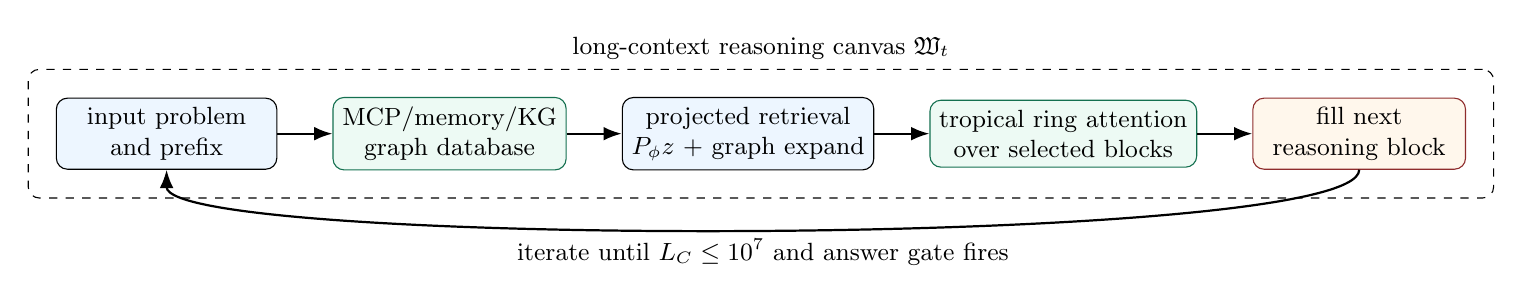
\begin{tikzpicture}[every node/.style={font=\small}, box/.style={draw, rounded corners, align=center, minimum height=0.85cm, fill=softblue}, gbox/.style={draw=darkgreen, rounded corners, align=center, fill=softgreen, minimum height=0.85cm}, obox/.style={draw=darkred, rounded corners, align=center, fill=softorange, minimum height=0.85cm}, arr/.style={-Latex, thick}]
\node[box, minimum width=2.8cm] (q) {input problem\\and prefix};
\node[gbox, right=0.7cm of q, minimum width=2.9cm] (db) {MCP/memory/KG\\graph database};
\node[box, right=0.7cm of db, minimum width=3.0cm] (retr) {projected retrieval\\$P_\phi z$ + graph expand};
\node[gbox, right=0.7cm of retr, minimum width=3.2cm] (ring) {tropical ring attention\\over selected blocks};
\node[obox, right=0.7cm of ring, minimum width=2.7cm] (fill) {fill next\\reasoning block};
\draw[arr] (q) -- (db);
\draw[arr] (db) -- (retr);
\draw[arr] (retr) -- (ring);
\draw[arr] (ring) -- (fill);
\draw[arr] (fill.south) .. controls +(0,-1.0) and +(0,-1.0) .. node[below]{iterate until $L_C\le 10^7$ and answer gate fires} (q.south);
\node[draw, dashed, rounded corners, fit=(q)(db)(retr)(ring)(fill), inner sep=0.35cm, label=above:{long-context reasoning canvas $\mathfrak{W}_t$}] {};
\end{tikzpicture}%
}
\caption{A 1--10M-token context is filled by repeated retrieval, tropical ring aggregation, and graph-structured reasoning blocks. The ring attention path gives exact max-plus provenance over selected or streamed blocks, while the projected retrieval path keeps search sublinear.}
\end{figure}

\subsection{Context tokens, graph tokens, and MCP records}
Let $\mathbb{D}$ be the external context database. It contains three interacting layers:
\begin{enumerate}
\item a raw layer of byte strings, markdown files, resource payloads, tool schemas, prompts, call/response traces, and knowledge-graph triples;
\item a graph layer $G_{\mathbb{D}}=(V,E)$ whose vertices are typed records and whose edges are containment, citation, temporal-successor, schema-field, capability, provenance, permission, entity-relation, and analogy links;
\item a vector/certificate layer with embeddings $z_v\in\RR^d$, projected vectors $u_v=P_\phi z_v\in\RR^r$, quantized codes $q_v$, sheaf sections $s_v$, filtered-complex memberships, toric chart ids, and small finite certificate summaries.
\end{enumerate}
The canvas $\mathfrak{W}_t$ is a finite excerpt of this database together with generated reasoning text. The excerpt may be large, but it is not arbitrary: it is produced by graph retrieval, permissions, context packing, and a final bits-per-byte gate.

\begin{definition}[Context incidence map]
A context incidence map is a function
\begin{equation}
\iota_t:I_t\longrightarrow V(G_{\mathbb{D}_t})\cup V_{\rm gen,t}
\end{equation}
from filled token positions to either database records or generated reasoning vertices. The map is compatible with adjacency when a token span from a record induces a connected interval in the context graph and when generated reasoning steps attach edges to the records they cite, transform, summarize, or verify.
\end{definition}

The incidence map is important for evaluation. If an answer cites a tool result, the answer tokens and the result tokens should have a short path in $G_{\mathbb{D}_t}$ and a compatible sheaf restriction. If a generated paragraph changes tone because of a style memory, the paragraph should be adjacent to that memory in the behavior subgraph. If the path is absent, the model may be using ungrounded latent memory rather than the retrieved context.

\subsection{Tropical ring attention over a full context}
Quadratic attention over $10^7$ tokens is not the intended primitive. ToricGT III uses a mixture of projected retrieval, sparse graph attention, and tropical ring attention. The tropical component is exact for max-plus aggregation and therefore ideal for provenance, active evidence, shortest-path-like reasoning, dynamic-programming recurrences, and hard evidence maxima.

Let $Q\in\RR^{m\times d}$ be a small query table, $K,V\in\RR^{L_C\times d}$ be key and value tables for a selected or streamed context, and let $\calB=\{B_1,\ldots,B_R\}$ be a partition of the context positions into blocks. For query $i$ and output channel $c$, define
\begin{equation}
Y_{ic}=\max_{1\le j\le L_C}\{\langle Q_i,K_j\rangle+V_{jc}+M_{ij}\},
\end{equation}
where $M_{ij}\in\{0,-\infty\}$ is a prefix, permission, type, or graph-sparsity mask.

\begin{definition}[Tropical ring summary]
The block summary for block $B_r$ is
\begin{equation}
Y^{(r)}_{ic}=\max_{j\in B_r}\{\langle Q_i,K_j\rangle+V_{jc}+M_{ij}\},
\end{equation}
with provenance set
\begin{equation}
A^{(r)}_{ic}=\argmax_{j\in B_r}\{\langle Q_i,K_j\rangle+V_{jc}+M_{ij}\}.
\end{equation}
A ring reducer passes summaries around a ring and computes
\begin{equation}
\bar Y_{ic}=\max_{r\le R}Y^{(r)}_{ic},\qquad \bar A_{ic}=\bigcup_{r:Y^{(r)}_{ic}=\bar Y_{ic}}A^{(r)}_{ic}.
\end{equation}
\end{definition}

\begin{theorem}[Exactness of tropical ring attention]
For any finite context length $L_C$, any partition $\calB$ of $\{1,\ldots,L_C\}$, any mask $M$, and any query/value channel $(i,c)$, the tropical ring summary satisfies
\begin{equation}
\bar Y_{ic}=Y_{ic},\qquad \bar A_{ic}=A_{ic}.
\end{equation}
The result is independent of the order in which blocks are reduced around the ring.
\end{theorem}
\begin{proof}
Because the blocks form a disjoint partition,
\begin{equation}
\max_{1\le j\le L_C} z_j=\max_{r\le R}\max_{j\in B_r} z_j
\end{equation}
for $z_j=\langle Q_i,K_j\rangle+V_{jc}+M_{ij}$. The binary maximum is associative and commutative, so ring order cannot change the exact real-arithmetic result. A position $j$ is a global maximizer if and only if it is a local maximizer in a block whose block value equals the global maximum. Hence the union rule gives exactly the global provenance set.
\end{proof}

\begin{corollary}[Streaming memory bound]
For $m$ query rows, $d$-dimensional keys, $c_o$ value channels, and block size $B$, exact tropical ring attention can be evaluated with working memory
\begin{equation}
O(Bd+mc_o+m c_o R_{\rm live})
\end{equation}
where $R_{\rm live}$ is the number of live block summaries retained for provenance. Without retaining full provenance, the working memory is $O(Bd+mc_o)$ plus the model state.
\end{corollary}
\begin{proof}
At any instant the evaluator needs the current block's keys/values, the query table, and running maxima. Exact provenance requires storing either all tied maximizers or a bounded top-$k$ summary. If only scores are needed, previous blocks can be discarded after their maxima are merged.
\end{proof}

\begin{definition}[Graph-sparse tropical ring attention]
Let $N_R(i)\subseteq \{1,\ldots,L_C\}$ be the context positions within graph radius $R$ of query position $i$ after permission filtering. The sparse mask is
\begin{equation}
M_{ij}^{\rm graph}=\begin{cases}0,&j\in N_R(i),\\ -\infty,&\text{otherwise.}\end{cases}
\end{equation}
Sparse ring attention is exact attention over the graph-admissible neighborhood and has work proportional to $\sum_i |N_R(i)|$ rather than $mL_C$.
\end{definition}

This distinction matters in a 10M-token setting. Full tropical scanning is useful for small $m$, global memory audits, or offline teacher passes. Online agents should usually retrieve a projected candidate set, expand it in the typed graph, and apply tropical ring attention to that induced subcontext plus a small set of global sentinel summaries.

\subsection{Soft attention, tropical attention, and answer probability}
Tropical ring attention is not a replacement for all soft attention. It is the exact primitive for active evidence and dynamic programming. Ordinary next-byte prediction still uses softmax or linear attention in the main model. The bridge is a side-channel: tropical summaries produce finite provenance codes and high-margin evidence features that condition ordinary logits.

\begin{definition}[Tropical evidence side-channel]
Given ring summaries $\bar Y$ and provenance $\bar A$, define a compact side code
\begin{equation}
\kappa_t=Q_{\rm code}\big(\bar Y_t,\;\mathrm{topk}(\bar A_t),\;\Delta_t,\;\mathrm{types}(\bar A_t),\;\mathrm{provenance}(\bar A_t)\big),
\end{equation}
where $\Delta_t$ is the top-two tropical margin. The next-byte model is
\begin{equation}
q_\theta(b_t\mid b_{<t},\mathfrak{W}_t)=\softmax\big(\ell_\theta(b_{<t})+R_\theta(\kappa_t,\mathfrak{W}_t)\big).
\end{equation}
\end{definition}

\begin{proposition}[Margin stability of tropical side codes]
Assume all key, query, and value perturbations change every candidate score by at most $\eps$. If the tropical top-two margin for $(i,c)$ is $\Delta_{ic}>2\eps$, then the active provenance set for a unique maximizer is unchanged under the perturbation.
\end{proposition}
\begin{proof}
Let $j^*$ be the unique maximizer and $j$ any competitor. Originally $z_{j^*}-z_j\ge \Delta_{ic}$. After perturbation, $\tilde z_{j^*}-\tilde z_j\ge \Delta_{ic}-2\eps>0$. Hence $j^*$ remains the unique maximizer.
\end{proof}

High-margin side codes are exactly the kind of finite structure that can survive quantization. Low-margin decisions should be routed to the teacher, a verifier, or a larger context expansion because they are unstable under projection and quantization.

\subsection{Learned projected retrieval for a 10M-token context}
The vector database contains high-dimensional vectors $z_v\in\RR^d$ and deployable projected vectors $u_v=P_\phi z_v\in\RR^r$ with $r\ll d$. A retrieval head must learn $P_\phi$ so that positives remain separated from hard negatives after projection and quantization.

\begin{definition}[Projected graph retrieval head]
For a query packet $x$ with embedding $z_x$, projected query $u_x=P_\phi z_x$, and database record $v$, define the projected score
\begin{equation}
S_\phi(x,v)=\langle P_\phi z_x, P_\phi z_v\rangle + \alpha\,\rho_\psi(x,v)+\beta\,g_\psi(x,v)-\gamma\,r_{\rm risk}(x,v),
\end{equation}
where $\rho_\psi$ is a typed relation score, $g_\psi$ is a graph-neighborhood score, and $r_{\rm risk}$ encodes permissions, stale provenance, unsafe tool surfaces, and behavior nonfaces. The ANN index stores $Q(P_\phi z_v)$, a quantized approximation of the projected vector.
\end{definition}

\begin{theorem}[Projection margin preservation]
Let $p$ be a useful context record and $n$ be a negative record for query $x$. Suppose the full score gap is
\begin{equation}
\langle z_x,z_p\rangle-\langle z_x,z_n\rangle\ge \Gamma.
\end{equation}
Assume the learned projection satisfies
\begin{equation}
|\langle P_\phi z_x,P_\phi z_v\rangle-\langle z_x,z_v\rangle|\le \eps_{\rm proj}
\end{equation}
for $v\in\{p,n\}$, and quantization adds at most $\eps_{\rm q}$ score error per item. If
\begin{equation}
\Gamma>2\eps_{\rm proj}+2\eps_{\rm q}+\eta_{\rm graph},
\end{equation}
where $\eta_{\rm graph}$ bounds graph/risk-score perturbation, then the projected quantized score still ranks $p$ above $n$.
\end{theorem}
\begin{proof}
The projected unquantized gap is at least $\Gamma-2\eps_{\rm proj}$. Quantization can reduce the positive score by $\eps_{\rm q}$ and increase the negative score by $\eps_{\rm q}$, giving a gap at least $\Gamma-2\eps_{\rm proj}-2\eps_{\rm q}$. Graph and risk terms can reduce it by at most $\eta_{\rm graph}$. The stated strict inequality leaves a positive gap.
\end{proof}

The theorem gives a practical training rule: mine hard negatives whose full-score gap is small, then train the projection and quantizer to enlarge the deployed margin on exactly those pairs. Easy positives do not teach the retrieval head how to survive compression.

\subsection{Quantized toric codes for context windows}
ToricGT III uses quantization for retrieval vectors, chart codes, and side-channel summaries. The toric component is useful because it separates roles: a token block can be represented by a Cox degree, a one-dimensional-cone chart id, a semigroup code, a Stanley-Reisner compatibility bitmask, and a residual vector. These codes are small and compositional.

\begin{definition}[Toric context code]
A toric context code for a record $v$ is
\begin{equation}
\chi(v)=(q_v,\;\deg_{\rm Cox}(v),\;\sigma(v),\;H(v),\;\Delta(v),\;\pi(v),\;s(v)),
\end{equation}
where $q_v$ is a product-quantized retrieval code, $\deg_{\rm Cox}(v)$ is a multidegree, $\sigma(v)$ is a cone or normal-fan cell id, $H(v)$ is a Hilbert-basis or semigroup-generator mask, $\Delta(v)$ is a filtered-complex signature, $\pi(v)$ is permission/provenance metadata, and $s(v)$ is a small sheaf-section summary.
\end{definition}

\begin{definition}[Toric code length]
The deployable code length of a context package $S$ is
\begin{equation}
\operatorname{bits}(\chi(S))=\sum_{v\in S}\operatorname{bits}(\chi(v))+\operatorname{bits}(E_S)+\operatorname{bits}(\mathrm{codebooks})+\operatorname{bits}(\mathrm{projection}).
\end{equation}
The code is admissible only if this length is counted in the artifact or runtime side-information budget.
\end{definition}

\begin{theorem}[Side-information criterion for context utility]
Let $Y$ be the future answer bytes, $X$ the visible prefix/problem, and $C$ a retrieved context package whose serialized side code has expected length $B(C)$ bits. If the model can use $C$ optimally and the code is prefix-visible, the expected net bit improvement is
\begin{equation}
I(Y;C\mid X)-B(C).
\end{equation}
Normalized by answer byte length $|Y|_{\rm byte}$, the retrieved context can improve bits-per-byte only if
\begin{equation}
\frac{I(Y;C\mid X)-B(C)}{|Y|_{\rm byte}}>0.
\end{equation}
\end{theorem}
\begin{proof}
Without $C$, the optimal expected code length for $Y$ given $X$ is $H(Y\mid X)$. With $C$ available and encoded at cost $B(C)$, it is $H(Y\mid X,C)+B(C)$. The difference is $H(Y\mid X)-H(Y\mid X,C)-B(C)=I(Y;C\mid X)-B(C)$. Dividing by answer bytes gives the bits-per-byte criterion.
\end{proof}

This theorem is the long-context version of the ToricGT deployment rule. A million extra tokens are not automatically helpful. They must carry more conditional information about future bytes, reasoning correctness, or behavior control than their representation costs.

\subsection{Filtered simplicial persistence of a growing context}
At iteration $t$, the canvas induces a filtered complex $\calK_t(\lambda)$. Vertices are context blocks, MCP records, markdown sections, KG entities, and generated reasoning steps. Edges encode adjacency, citation, schema compatibility, temporal succession, graph relation, or retrieval coactivation. Higher simplices encode mutually compatible sets of evidence, tools, claims, or behavior factors.

\begin{definition}[Growing context filtration]
A growing context filtration is a bifiltration
\begin{equation}
\calK_{t,\lambda}\subseteq \calK_{t',\lambda'}\quad\text{whenever}\quad t\le t'\;\text{and}\;\lambda\le \lambda',
\end{equation}
where $t$ is reasoning time and $\lambda$ is an evidence, confidence, distance, or relevance threshold. The associated persistence module is
\begin{equation}
M_i(t,\lambda)=H_i(\calK_{t,\lambda};\FF).
\end{equation}
\end{definition}

\begin{proposition}[Monotone fill gives functorial persistence]
If the fill trajectory is monotone and thresholds are nested, then $(t,\lambda)\mapsto H_i(\calK_{t,\lambda};\FF)$ is a functor from the poset $([T]\times\Lambda,\le)$ to finite-dimensional vector spaces.
\end{proposition}
\begin{proof}
A monotone fill gives inclusions of complexes $\calK_{t,\lambda}\hookrightarrow \calK_{t',\lambda'}$ whenever $(t,\lambda)\le(t',\lambda')$. Homology is functorial with respect to inclusions, and composition of inclusions maps to composition of homology maps. Thus the assignment is a persistence module.
\end{proof}

When memory edits delete or rewrite blocks, inclusions may fail. Then the correct object is a zigzag module. This is common for MCP agents: an unsafe retrieval may be removed after a permission check; a stale memory may be replaced; a tool result may be superseded. ToricGT III logs both the monotone teacher view and the deployment zigzag view.

\begin{definition}[Context persistence drift]
Let $D_i(t)$ be the persistence diagram or a finite barcode summary of $H_i(\calK_{t,\lambda})$ over $\lambda$. The long-context topology drift is
\begin{equation}
\loss_{\rm pers\mbox{-}drift}=\sum_{t<\tau_C}d_B(D_i(t),D_i(t+1))^2
\end{equation}
with $d_B$ the bottleneck distance, or a differentiable sliced-Wasserstein surrogate.
\end{definition}
A low drift is not always desirable. Hard problems require phase changes. The useful target is \emph{explained} drift: topology may change when new evidence, a tool result, or a proof branch enters, but not because of unstable retrieval noise or style drift.

\subsection{Sheaves and global sections over a long window}
A 10M-token canvas is too large to trust by surface recency alone. It needs local-to-global checks. The sheaf language is a compact way to express them. A local section may be the factual content of a resource block, a tool schema, a table row, a proof obligation, a behavior profile, a citation cluster, or a memory entry. Adjacent sections must agree on overlaps.

\begin{definition}[Context sheaf over a reasoning canvas]
Let $\calK_t$ be the context complex. A context sheaf $\calF_t$ assigns a vector space, lattice, finite set, or structured record $\calF_t(\sigma)$ to each simplex $\sigma\in\calK_t$, together with restriction maps
\begin{equation}
\rho_{\tau\sigma}:\calF_t(\sigma)\to\calF_t(\tau),\qquad \tau\subseteq\sigma,
\end{equation}
such that $\rho_{\upsilon\tau}\rho_{\tau\sigma}=\rho_{\upsilon\sigma}$ whenever $\upsilon\subseteq\tau\subseteq\sigma$.
\end{definition}

\begin{definition}[Long-context global section residual]
Given predicted local sections $s_\sigma\in\calF_t(\sigma)$, the Cech gluing residual is
\begin{equation}
\loss_{\check C,t}=\sum_{\tau\subseteq\sigma}\|\rho_{\tau\sigma}s_\sigma-s_\tau\|^2.
\end{equation}
For a trajectory, use the length-normalized loss
\begin{equation}
\loss_{\check C}^{\rm long}=\frac1{\max(1,L_C)}\sum_{t<\tau_C}\sum_{\tau\subseteq\sigma\in\calK_t}\|\rho_{\tau\sigma}s^t_\sigma-s^t_\tau\|^2.
\end{equation}
\end{definition}

\begin{theorem}[Zero Cech residual gives compatible context]
If $\loss_{\check C,t}=0$, then the local sections form a compatible family. If $\calF_t$ is a sheaf on the finite complex topology, this family determines a unique global section over the union of the covered context cells whenever the cover is jointly epimorphic in the usual sheaf sense.
\end{theorem}
\begin{proof}
The equality $\rho_{\tau\sigma}s_\sigma=s_\tau$ for every inclusion is precisely the compatibility condition for local sections. The sheaf axiom says that compatible local sections over a cover glue uniquely to a global section. On a finite complex, the statement reduces to equalizer conditions over intersections; zero residual enforces those equalities.
\end{proof}

This is useful for accuracy and tone. Factual claims should glue across cited resources; tool descriptions should glue with actual tool results; a user's preferred register should glue across markdown memory and current answer; uncertainty should restrict consistently from global answer to individual claims.

\subsection{Derived updates for MCP and memory edits}
The context database is dynamic. A tool result may refine a claim, a markdown memory may split, and a knowledge-graph entity may merge with another. Derived language gives a precise error signal for whether an update preserves the intended information.

\begin{definition}[Context update complex]
Let $C_t^\bullet$ be a cochain complex built from the context sheaf, persistence module, or free resolution at time $t$. A learned update produces a chain map candidate
\begin{equation}
f_t:C_t^\bullet\to C_{t+1}^\bullet.
\end{equation}
The update-cone residual is the homology or rank profile of the mapping cone $\operatorname{Cone}(f_t)$.
\end{definition}

\begin{theorem}[Mapping-cone criterion]
A chain map $f:C^\bullet\to D^\bullet$ is a quasi-isomorphism if and only if $\operatorname{Cone}(f)$ is acyclic.
\end{theorem}
\begin{proof}
The mapping cone fits into a distinguished triangle $C^\bullet\to D^\bullet\to \operatorname{Cone}(f)\to C^\bullet[1]$. The associated long exact sequence in cohomology shows that $H^k(f):H^k(C)\to H^k(D)$ is an isomorphism for all $k$ exactly when $H^k(\operatorname{Cone}(f))=0$ for all $k$.
\end{proof}

In practice, exact acyclicity is teacher-side. The deployable signal is a small vector: ranks, Betti summaries, cone homology dimensions, and a confidence margin. A memory rewrite is accepted when it improves utility while keeping the cone residual below the task-specific threshold.

\subsection{Ergodic theory of long-context fill dynamics}
The long-context fill process is a controlled dynamical system. Even when the raw context space is huge, the quantized deployment state is finite: projected vector codes, chart ids, behavior alcoves, permission masks, and small certificate summaries all lie in finite codebooks.

\begin{definition}[Quantized fill state]
A quantized fill state is
\begin{equation}
\bar S_t=(\bar c_t,\bar g_t,\bar k_t,\bar f_t,\bar b_t,\bar r_t),
\end{equation}
where $\bar c_t$ is a context-pack code, $\bar g_t$ is a graph-neighborhood code, $\bar k_t$ is a filtered-complex signature, $\bar f_t$ is a sheaf-gluing signature, $\bar b_t$ is a behavior-corridor cell, and $\bar r_t$ is a retrieval/provenance signature. The learned policy and environment induce a Markov kernel on the finite set of possible $\bar S_t$.
\end{definition}

\begin{theorem}[Finite long-context recurrence]
For fixed codebooks, bounded database capacity, bounded context length $C_{\max}$, and deterministic decoding temperature $0$, every quantized fill trajectory is eventually periodic. For stochastic decoding, the process is a finite Markov chain and admits at least one stationary distribution.
\end{theorem}
\begin{proof}
In the deterministic case, a map from a finite set to itself must revisit a state; after the first repeated state, the trajectory cycles. In the stochastic case, the transition kernel is a finite stochastic matrix, which has a stationary distribution by compactness of the probability simplex.
\end{proof}

\begin{definition}[Long-context ergodic observables]
Important observables include
\begin{align}
\varphi_{\rm bits-per-byte}(\bar S_t)&=\text{local held-out bits-per-byte},\\
\varphi_{\rm ret}(\bar S_t)&=\text{retrieval precision or recall at budget},\\
\varphi_{\rm tone}(\bar S_t)&=\text{tone/personality corridor distance},\\
\varphi_{\rm acc}(\bar S_t)&=\text{verifier disagreement or hallucination score},\\
\varphi_{\rm risk}(\bar S_t)&=\text{permission, privacy, or tool-safety violation score},\\
\varphi_{\rm topo}(\bar S_t)&=\text{persistence, Cech, or mapping-cone residual}.
\end{align}
\end{definition}

The empirical long-run profile
\begin{equation}
\hat\Phi_T=\frac1T\sum_{t=0}^{T-1}(\varphi_{\rm bits-per-byte},\varphi_{\rm ret},\varphi_{\rm tone},\varphi_{\rm acc},\varphi_{\rm risk},\varphi_{\rm topo})(\bar S_t)
\end{equation}
selects cache policy. States with high recurrence, high information gain, and low risk become persistent compressed memory. States with high recurrence but high verifier or safety loss become forbidden or require confirmation.

\subsection{Stopping, sufficiency, and context length control}
A long context agent should not always fill the maximum window. The correct stopping rule balances answer certainty, context cost, and expected information gain.

\begin{definition}[Context sufficiency score]
Let $p_\theta(a\mid q,\mathfrak{W}_t)$ be the answer distribution, $v_\psi$ a verifier score, $r_\psi$ a retrieval uncertainty score, and $c_t=L(\mathfrak{W}_t)/C_{\max}$. Define
\begin{equation}
\operatorname{Suff}_t=\alpha\,v_\psi(q,a_t,\mathfrak{W}_t)-\beta\,H(p_\theta(\cdot\mid q,\mathfrak{W}_t))-\gamma\,r_\psi(q,\mathfrak{W}_t)-\delta\,c_t.
\end{equation}
The answer gate fires when $\operatorname{Suff}_t\ge\kappa$ and all mandatory schema, provenance, permission, and behavior checks pass.
\end{definition}

\begin{proposition}[One-step stopping criterion]
Let $G_t$ be the expected future gain in answer log score from one more context-fill step and let $K_t$ be the expected token/runtime/side-code cost measured in bits. A myopic stop is optimal among stop/continue for one additional step when
\begin{equation}
G_t\le K_t.
\end{equation}
\end{proposition}
\begin{proof}
Continuing changes expected net code length by $K_t-G_t$. If this quantity is nonnegative, one more step does not improve the one-step net objective. If it is negative, the expected net code length decreases and continuing is myopically preferable.
\end{proof}

This criterion should be trained as a calibration target: many hard tasks need far less than 10M tokens, while some multi-file MCP tasks require a large context. The agent should learn problem-dependent $L_C$ rather than defaulting to maximum context.

\subsection{Implementation for a 1--10M-token MCP/memory/KG agent}
A practical system separates raw storage, graph retrieval, long-context streaming, and exact audits.
\begin{lstlisting}[language=Python,caption={Long-context ToricGT III retrieval and fill loop.}]
def solve_with_long_context(problem, db, C_max=10_000_000):
    W = init_canvas(problem, C_max=C_max)
    state = init_reasoning_state(problem)
    while W.filled_tokens < C_max:
        q = query_packet(problem, W, state)
        # 1. Fast projected vector search.
        u = P_phi @ query_encoder(q)
        seeds = ann_index.topk(quantize(u), k=K_seed)
        # 2. Typed graph expansion with permission and safety filters.
        subgraph = expand_graph(db.graph, seeds, radius=R,
                                permissions=q.permissions,
                                nonfaces=SR_behavior_rules)
        # 3. Build streamed blocks from MCP, markdown, KG, and generated steps.
        blocks = pack_blocks(subgraph, W.remaining_budget,
                             scores=projected_scores(u, subgraph))
        # 4. Exact max-plus provenance over streamed blocks.
        trop = tropical_ring_attention(q.hidden_queries, stream(blocks),
                                       masks=prefix_permission_graph_masks)
        # 5. Ordinary decoder uses compact side-channel and selected text.
        delta, state = model_fill_step(problem, W, state, blocks, trop.side_code)
        W.append(delta)
        # 6. Stop when answer sufficiency beats expected context gain.
        if answer_gate(problem, W, state):
            break
    return render_answer(W, state), audit_trace(W, state)
\end{lstlisting}

The index should store at least five arrays: projected quantized vectors for ANN; CSR adjacency by typed relation; block offsets into raw text or MCP payloads; compact toric context codes; and permission/provenance masks. Exact sheaf, resolution, and persistence objects can be computed in a teacher-side audit process and distilled into small summaries.

\subsection{Long-context training data construction}
Training examples should include both short and long contexts. A record has the form
\begin{equation}
(q,\;\mathbb{D}_0,\;\{\mathfrak{W}_t\}_{t\le \tau_C},\;a,\;\calA),
\end{equation}
where $\calA$ is an audit package containing retrieval positives, negatives, tool permissions, schema labels, evidence paths, markdown gluing labels, KG proof paths, verifier judgments, and optional algebraic certificates.

Useful synthetic families include: multi-hop knowledge-graph proofs with distractor communities; MCP tool-use tasks with schema-compatible and schema-incompatible tools; markdown project-memory tasks requiring a style profile plus factual recall; long mathematical derivations with tableaux or root-system subproblems; codebase navigation tasks where repository files are graph nodes; and safety tasks in which relevant information is present but permission or policy nonfaces block direct use.

The data curriculum should scale $L_C$ in phases:
\begin{equation}
2^{12}\to 2^{14}\to 2^{16}\to 2^{18}\to 2^{20}\to 10^6\to 10^7.
\end{equation}
At each phase, keep a fixed short-context slice. A long-context method that improves 10M-token tasks but damages short ordinary text is not ready for deployment without a gate.

\section{Long-context objective catalogue}
The previous objective catalogue remains valid for graph databases. This section adds objectives designed specifically for a 1--10M-token iterative context canvas. Each objective is audit-first; it becomes train-time only after exact finite checks agree with the differentiable surrogate, and it becomes deployable only after held-out bits-per-byte or predeclared reasoning/control metrics improve under artifact accounting.

\subsection{LC1. Context Canvas Bits-per-Byte Utility}
\textbf{Definition.} For a context package $C_t\subset\mathbb{D}_t$ and answer bytes $Y$, define
\begin{equation}
U_{\rm canvas}(C_t)=\frac{1}{|Y|_{\rm byte}}\left[\log_2\frac{q_\theta(Y\mid X,C_t)}{q_\theta(Y\mid X)}-\operatorname{bits}(\chi(C_t))\right].
\end{equation}
\textbf{Why it helps.} This is the direct long-context utility. It rejects context that is semantically attractive but entropy-increasing after serialization. \textbf{Integration.} Use it as an offline label for context packers and as a reward for GFlowNet context selection. Train on matched examples with and without $C_t$ to avoid confounding.

\subsection{LC2. Tropical Ring Provenance Margin Loss}
\textbf{Definition.} Let $\Delta_{ic}=z^{(1)}_{ic}-z^{(2)}_{ic}$ be the top-two tropical margin. Use
\begin{equation}
\loss_{\rm ring\mbox{-}margin}=\sum_{i,c}\max(0,\gamma-\Delta_{ic})\,w_{ic},
\end{equation}
where $w_{ic}$ is high only for channels whose provenance is verified useful. \textbf{Why it helps.} High tropical margins make provenance robust under projection, block streaming, and quantization. \textbf{Integration.} Attach to evidence maxima, tool-choice maxima, active KG paths, and proof obligations. Do not apply globally; low margins are valid when the task is genuinely ambiguous.

\subsection{LC3. Projected Retrieval Gap Preservation}
\textbf{Definition.} For positives $p$ and hard negatives $n$, train
\begin{equation}
\loss_{\rm proj\mbox{-}gap}=\max\left(0,\gamma-S_\phi(x,p)+S_\phi(x,n)\right).
\end{equation}
\textbf{Why it helps.} The full database cannot be searched exactly at every step. The projected head must preserve useful ordering under dimension reduction. \textbf{Integration.} Mine negatives from same markdown file, same tool family, same KG relation type, and same behavior alcove.

\subsection{LC4. Quantized Score Robustness}
\textbf{Definition.} If $\hat z_v$ reconstructs $P_\phi z_v$ from a codebook, penalize
\begin{equation}
\loss_{\rm qscore}=\sum_{(x,v)}\left(\langle P_\phi z_x,P_\phi z_v\rangle-\langle \hat z_x,\hat z_v\rangle\right)^2.
\end{equation}
\textbf{Why it helps.} A retrieval head that works only before quantization is not a deployable retrieval head. \textbf{Integration.} Use fake quantization during training and exact codebook reconstruction during validation.

\subsection{LC5. Graph Expansion Recall Objective}
\textbf{Definition.} Let $E_R(C)$ be the radius-$R$ expansion of ANN seeds. Train the seed retriever so that
\begin{equation}
\loss_{\rm expand}= -\log \Pr[P(x)\cap E_R(C_k(x))\ne\emptyset].
\end{equation}
\textbf{Why it helps.} For very large contexts, the seed need not be the exact record if it lands near the useful subgraph. \textbf{Integration.} Label positive neighborhoods, not only positive chunks. This is essential for KG and codebase retrieval.

\subsection{LC6. MCP Capability Nonface Barrier}
\textbf{Definition.} If $\Delta_{\rm MCP}$ is the allowed capability complex, penalize forbidden coactivation
\begin{equation}
\loss_{\rm MCP\mbox{-}SR}=\sum_{F\notin\Delta_{\rm MCP}}\prod_{i\in F}p_i.
\end{equation}
\textbf{Why it helps.} Tool descriptors, private resources, and code-execution paths must not be combined merely because they are relevant. \textbf{Integration.} Use MCP permissions and tool-safety labels to build nonfaces; evaluate on adversarial tool-description tasks.

\subsection{LC7. Markdown Cech Memory Gluing}
\textbf{Definition.} For markdown blocks $U_i$ and overlaps $U_i\cap U_j$, use
\begin{equation}
\loss_{\rm md\mbox{-}\check C}=\sum_{i<j}\|s_i|_{U_{ij}}-s_j|_{U_{ij}}\|^2.
\end{equation}
\textbf{Why it helps.} Long-context agents often retrieve inconsistent versions of project memory. Cech gluing detects contradiction before generation. \textbf{Integration.} Build overlaps from headings, anchors, backlinks, timestamps, and citations.

\subsection{LC8. KG Path Sheaf Consistency}
\textbf{Definition.} For two KG paths $p_1,p_2$ supporting the same claim, compare transported sections:
\begin{equation}
\loss_{\rm KG\mbox{-}path}=\|T_{p_1}s_{\rm source}-T_{p_2}s_{\rm source}\|^2.
\end{equation}
\textbf{Why it helps.} Multi-hop reasoning should not depend on arbitrary path choice unless the paths encode genuinely different evidence. \textbf{Integration.} Use relation-specific transports and train on symmetric, inverse, transitive, and typed relation families.

\subsection{LC9. Long-Context Occupation Entropy Regularizer}
\textbf{Definition.} Let $\hat\mu_T(c)$ be occupation of quantized context cells. Penalize collapse or chaos by
\begin{equation}
\loss_{\rm occ}=\left(H(\hat\mu_T)-H_{\rm target}\right)^2.
\end{equation}
\textbf{Why it helps.} A long context agent should reuse stable states without collapsing to the same retrieval pattern for every task. \textbf{Integration.} Estimate on task slices; set $H_{\rm target}$ differently for deterministic algebra tasks and exploratory research tasks.

\subsection{LC10. Recurrence Utility Cache Loss}
\textbf{Definition.} For a context cell $c$, define cache utility
\begin{equation}
U_{\rm cache}(c)=\hat\mu(c)\,\Delta\bitsperbyte(c)-\lambda_{\rm risk}R(c)-\lambda_{\rm bytes}\operatorname{bits}(c).
\end{equation}
\textbf{Why it helps.} Frequently reused helpful states deserve compact persistent codes; frequently reused harmful states should be gated. \textbf{Integration.} Use this to promote records from raw memory to quantized fast memory.

\subsection{LC11. Context Packing Submodularity Loss}
\textbf{Definition.} For learned utility $U(S)$, penalize violations of diminishing returns:
\begin{equation}
\loss_{\rm submod}=\sum_{A\subseteq B,\,v\notin B}\max(0,\Delta_v(B)-\Delta_v(A))^2.
\end{equation}
\textbf{Why it helps.} Approximate submodularity makes greedy context packing reliable under token budgets. \textbf{Integration.} Sample small sets $A,B$ from candidate packs; do not require exact submodularity for all context.

\subsection{LC12. Reasoning Fill Monotonicity and Zigzag Alarm}
\textbf{Definition.} For monotone phases, penalize deletion of required support:
\begin{equation}
\loss_{\rm fill}=\sum_t \|\mathbf{1}_{I_t}\odot(1-\mathbf{1}_{I_{t+1}})\|_1.
\end{equation}
For edit phases, log a zigzag alarm when deletion changes persistence beyond threshold. \textbf{Why it helps.} The model should not silently forget evidence already used in a proof. \textbf{Integration.} Allow explicit memory rewrite actions, but require mapping-cone and verifier audits.

\subsection{LC13. Derived Update Cone Loss}
\textbf{Definition.} For update chain map $f_t:C_t^\bullet\to C_{t+1}^\bullet$, use
\begin{equation}
\loss_{\rm cone}=\sum_k \dim H^k(\operatorname{Cone}(f_t))
\end{equation}
when exact, or a differentiable rank surrogate. \textbf{Why it helps.} It distinguishes information-preserving summarization from destructive memory rewrite. \textbf{Integration.} Use exact finite-field audits offline and low-rank surrogates online.

\subsection{LC14. Persistence Event Explanation Loss}
\textbf{Definition.} Let $e_t$ be an event label: new evidence, tool result, contradiction, permission removal, or style memory. Train
\begin{equation}
\loss_{\rm event}=\CE(e_t,\hat e_t)+\lambda\|\Delta D_t-R_{e_t}\|^2,
\end{equation}
where $\Delta D_t$ is barcode change and $R_{e_t}$ is the expected pattern. \textbf{Why it helps.} Topological drift is useful only when explained by an actual reasoning event. \textbf{Integration.} Label synthetic long-context tasks with known evidence arrivals.

\subsection{LC15. Tone/Personality Global Section Loss}
\textbf{Definition.} Let $b_\sigma$ be behavior sections over context cells. Use
\begin{equation}
\loss_{\rm tone\mbox{-}global}=\sum_{\tau\subseteq\sigma}\|\rho_{\tau\sigma}b_\sigma-b_\tau\|^2+\lambda\sum_t\dist(b_t,K_{\rm task})^2.
\end{equation}
\textbf{Why it helps.} Tone and personality drift across a 10M-token trajectory can degrade user trust and accuracy. \textbf{Integration.} Apply to style memories, current user instructions, safety state, and answer sections.

\subsection{LC16. Evidence Boundary Accuracy Loss}
\textbf{Definition.} For each answer claim $a_j$, let $\partial a_j$ be its required evidence boundary. Penalize missing support:
\begin{equation}
\loss_{\rm evidence}=\sum_j\max(0,\gamma-\operatorname{support}(\partial a_j,\mathfrak{W}_{\tau_C})).
\end{equation}
\textbf{Why it helps.} Long context increases hallucination risk unless claims are tied to retrieved evidence. \textbf{Integration.} Use verifier-generated claim/evidence pairs and KG path labels.

\subsection{LC17. Tool-Call Schema Degree Loss}
\textbf{Definition.} Assign each tool-call argument a Cox-like degree. Penalize degree mismatch:
\begin{equation}
\loss_{\rm schema\mbox{-}deg}=\sum_a \|\deg(a)-\deg_{\rm schema}(a)\|_1+\lambda\,\mathbf{1}\{\text{invalid JSON/schema}\}.
\end{equation}
\textbf{Why it helps.} It makes tool validity a typed algebraic constraint rather than a surface format afterthought. \textbf{Integration.} Train on MCP tool schemas with adversarial near-valid calls.

\subsection{LC18. Privacy and Permission Ideal Loss}
\textbf{Definition.} Let $I_{\rm priv}$ be an ideal or monomial nonface set generated by forbidden combinations of private resources, tools, and outputs. Use
\begin{equation}
\loss_{\rm priv}=\sum_{x^F\in I_{\rm priv}}\prod_{i\in F}p_i.
\end{equation}
\textbf{Why it helps.} Relevance does not imply permission. This loss blocks unsafe context joins. \textbf{Integration.} Use host/client/server permission boundaries and consent labels.

\subsection{LC19. Tropical Segment-Tree Distillation}
\textbf{Definition.} Let $T_{\rm full}$ be full tropical ring output and $T_{\rm seg}$ be a compressed segment tree of block summaries. Train
\begin{equation}
\loss_{\rm seg}=\|T_{\rm full}-T_{\rm seg}\|^2+\lambda\,d_{\rm prov}(A_{\rm full},A_{\rm seg}).
\end{equation}
\textbf{Why it helps.} Segment summaries let a 10M-token context expose global evidence without rescanning every token. \textbf{Integration.} Use teacher scans to train persistent block summaries.

\subsection{LC20. Answer Stopping-Time Efficiency}
\textbf{Definition.} With terminal time $\tau_C$, answer quality $Q$, and context cost $L_C$, train
\begin{equation}
\loss_{\rm stop}= -Q(a,\mathfrak{W}_{\tau_C})+\lambda\frac{L_C}{C_{\max}}+\eta\max(0,\kappa-\operatorname{Suff}_{\tau_C}).
\end{equation}
\textbf{Why it helps.} The agent should use 10M tokens only when the problem requires them. \textbf{Integration.} Train on tasks with known minimal evidence sets and evaluate quality as a function of allowed context length.

\section{Training objectives and losses}
\subsection{Base objective}
The base objective is always the prequential byte loss, written explicitly as bits-per-byte:
\begin{equation}
\loss_{\bitsperbyte}(\theta)=-\frac1T\sum_{t=1}^T\log_2 q_\theta(b_t\mid b_{<t},\operatorname{retrieve}_{<t}).
\end{equation}
Retrieval must be prefix-safe. Auxiliary losses are staged:
\begin{equation}
\loss=\loss_{\bitsperbyte}+\lambda_r\loss_{\rm retr}+\lambda_g\loss_{\rm graph}+\lambda_s\loss_{\rm sheaf}+\lambda_q\loss_{\rm quant}+\sum_j\lambda_j\loss_j.
\end{equation}
The deployment gate is
\begin{equation}
\lambda_j>0\Rightarrow \Delta\bitsperbyte_j> -\delta,\quad \mathrm{audit}_j=1,\quad \mathrm{artifact}_j\le A_{\max},\quad \mathrm{security}_j=\mathrm{pass}.
\end{equation}

\subsection{Core retrieval objective}
For a query $x$, positives $P(x)$, hard negatives $N(x)$, and a candidate set $C=P(x)\cup N(x)$, the retrieval objective is
\begin{equation}
\loss_{\rm retr}(x)=-\log \frac{\sum_{v\in P(x)}\exp S(x,v)/\tau}{\sum_{u\in C}\exp S(x,u)/\tau}.
\end{equation}
Graph smoothness and typed relation calibration are
\begin{align}
\loss_{\rm lap}&=\sum_{(u,v)\in E}w_{uv}\|z_u-R_{\tau(u,v)}z_v\|^2,\\
\loss_{\rm rel}&=\sum_{(u,\tau,v)}\max(0,\gamma+\|z_u+R_\tau-z_v\|^2-\|z_u+R_{\tau'}-z_{v'}\|^2).
\end{align}
The graph-structured objective is
\begin{equation}
\loss_{\rm gdb}=\loss_{\rm retr}+\lambda_{\rm lap}\loss_{\rm lap}+\lambda_{\rm rel}\loss_{\rm rel}+\lambda_{\check C}\loss_{\check C}+\lambda_{\rm form}\loss_{\rm form}+\lambda_{\rm tq}\loss_{\rm tq}.
\end{equation}

\subsection{Forty objectives for ToricGT III}
The catalogue has two parts. Part I adapts the best ToricGT II objectives to MCP/memory/KG retrieval. Part II introduces objectives native to graph-structured vector databases and protocol-safe context systems. Each item includes a mathematical object, loss or metric, reason it can improve bits-per-byte or reasoning, and integration notes.

\small
\begin{longtable}{p{0.05\textwidth}p{0.31\textwidth}p{0.56\textwidth}}
\toprule
ID & Objective & Primary role in ToricGT III\\
\midrule
\endhead
A1 & Context side-information bits-per-byte gate & Promote MCP/memory/KG certificates only when prefix-visible retrieval improves held-out bits-per-byte or verified reasoning.\\
A2 & MCP certificate conditional information & Estimate $I(B_t;Z_t\mid\mathcal{F}_t)$ for tool/resource/memory codes; suppress decorative retrieval metadata.\\
A3 & Protocol active-cell entropy margin & Stabilize tool/resource/prompt active regions in projected retrieval space.\\
A4 & Saturated semigroup memory code & Remove missing-code holes in quantized metadata and context-role algebra.\\
A5 & Hilbert-basis context primitive sparsity & Store reusable minimal context primitives rather than redundant long traces.\\
A6 & Toric-ideal KG path consistency & Enforce equivalent relation paths and schema compositions to score similarly.\\
A7 & Cox-degree role conservation & Preserve evidence, verifier, style, memory, tool, and answer-commitment degrees through retrieval.\\
A8 & Cartier support-function retrieval slope & Share local ranking slopes across equivalent context charts.\\
A9 & Moment-map context summary quantizer & Convert active retrieval geometry into a compact moment vector.\\
A10 & Stanley-Reisner forbidden context nonfaces & Penalize incompatible coactivations such as low evidence plus high confidence or unsafe tool plus no consent.\\
A11 & Cech markdown-memory gluing & Detect and penalize incompatible local memory sections.\\
A12 & Vector-bundle behavior transport & Maintain coherent tone, persona, rigor, and refusal axes across retrieved contexts.\\
A13 & Filtration-bundle expert retrieval & Route query types to specialized retrieval subbundles while sharing a compact base representation.\\
A14 & Closed differential-form evidence flow & Enforce path-independent evidence accumulation in retrieved support graphs.\\
A15 & Secondary-fan schema migration & Control schema wall crossings when MCP servers or memory formats change.\\
A16 & Gale-dual tool/resource pairing & Pair tools with dual resources or diagnostics to improve transfer and audit.\\
A17 & Young-tableau ontology compression & Canonicalize hierarchical entity schemas, task decompositions, and output templates.\\
A18 & Littlewood-Richardson context composition & Supervise branch-merge retrieval plans by associative combinatorial composition.\\
A19 & Derived memory-update chain map & Measure database updates by mapping-cone residuals.\\
A20 & Ergodic context Pareto controller & Gate long-run tradeoffs among bits-per-byte, retrieval, verifier, latency, safety, and artifact bytes.\\
N1 & MCP trace graph reconstruction & Train embeddings to reconstruct event types, call-return edges, schemas, and permissions.\\
N2 & Markdown heading sheaf exactness & Make local summaries and retrieved section data glue across heading overlaps.\\
N3 & Tool/resource schema preservation & Ensure projected vectors preserve JSON-schema and output-schema compatibility.\\
N4 & Graph-structured ANN recall & Train projection and quantization for high recall after graph expansion.\\
N5 & Projection distortion margin loss & Penalize hard-pair inner-product distortion near retrieval decision boundaries.\\
N6 & Quantized adjacency-aware retrieval & Train vector codes jointly with typed adjacency and path features.\\
N7 & Context-packing submodular utility & Select compact context packages maximizing predicted utility under token and artifact budgets.\\
N8 & Provenance residue safety loss & Treat unresolved provenance or consent obligations as logarithmic boundary residues.\\
N9 & Tool-call return cycle consistency & Check that tool outputs answer the schema and semantic intent of the call.\\
N10 & Prompt-template section distillation & Distill reusable prompt templates as sections over task charts.\\
N11 & KG path-algebra normal form & Canonicalize relation paths and suppress spurious equivalent paths.\\
N12 & Simplicial coactivation memory nonfaces & Use a Stanley-Reisner ideal to reject incoherent retrieved memory packages.\\
N13 & Local-cohomology conflict alarm & Use local obstruction classes to flag contradictions and missing context.\\
N14 & MCP cache spectral-gap controller & Tune cache refresh and eviction using mixing and recurrence diagnostics.\\
N15 & Retrieval trace entropy-rate loss & Reduce irrelevant retrieval oscillation without collapsing useful exploration.\\
N16 & Memory update mapping-cone residual & Quantify whether edits preserve or intentionally change derived context structure.\\
N17 & Derived index compaction & Compress Betti/resolution signatures for fast retrieval-side comparison.\\
N18 & Toroidal periodic context cache & Use phase codes for recurring tasks, cron-like tools, and periodic memories.\\
N19 & Behavior-corridor memory sheaf & Store tone/personality and accuracy controls as sheaf sections over memories.\\
N20 & Artifact-budget context controller & Decide what retrieval heads, codes, and certificates enter the deployable artifact.\\
\bottomrule
\end{longtable}
\normalsize

\clearpage
\subsection{Part I: adapted ToricGT objectives}

\Needspace{8\baselineskip}\paragraph{A1. Context side-information bits-per-byte gate.}
\textbf{Object.} Prefix-safe MCP or memory certificate $Z_t$, such as a tool schema code, sheaf-gluing flag, graph path signature, or quantized toric chart code. \textbf{Loss/metric.}
\begin{equation}
\Delta \bitsperbyte(Z)=\frac1T\sum_t\log_2\frac{q_\theta(b_t\mid\mathcal{F}_t,Z_t)}{q_0(b_t\mid\mathcal{F}_t)}-\lambda_A\operatorname{bytes}(Z)-\lambda_L\operatorname{latency}(Z).
\end{equation}
\textbf{Why it helps.} This is the promotion controller. It prevents MCP machinery from becoming a decorative retrieval stack. A certificate is useful only if it lowers conditional byte entropy or a predeclared verified-reasoning slice without exceeding artifact and latency budgets. \textbf{Integration.} Run base, shuffled-certificate, teacher-certificate, and quantized-student ablations. Promote only if exact audits pass and held-out bits-per-byte is nondegrading.

\Needspace{8\baselineskip}\paragraph{A2. MCP certificate conditional information.}
\textbf{Object.} A finite code $Z$ for retrieved context: source, schema, tool, heading, KG motif, persistence barcode, or Cech status. \textbf{Metric.} Estimate conditional information with a held-out classifier or likelihood ratio:
\begin{equation}
\widehat I(B;Z\mid C)=\frac1n\sum_i \log_2\frac{\hat q(b_i\mid c_i,z_i)}{\hat q(b_i\mid c_i)}.
\end{equation}
\textbf{Why it helps.} It tells whether the retrieval structure predicts the next bytes, not whether it looks coherent in isolation. \textbf{Integration.} Use it for probe selection and logging. Do not backpropagate aggressively until matched-seed bits-per-byte lift is observed.

\Needspace{8\baselineskip}\paragraph{A3. Protocol active-cell entropy margin.}
\textbf{Object.} Normal-fan cells in projected query space, induced by affine retrieval candidates. \textbf{Loss.}
\begin{equation}
\loss_{\rm cell}=H(C_t\mid \mathrm{task})+\lambda\,\mathbb E\max(0,\gamma-m_t),
\end{equation}
where $C_t$ is active cell id and $m_t$ is top-two cell margin. \textbf{Why it helps.} Stable cells make tool/resource selection predictable and reduce context jitter. \textbf{Integration.} Audit against exact cell ids after rationalizing candidate slopes; reject if entropy drops by collapse rather than better retrieval.

\Needspace{8\baselineskip}\paragraph{A4. Saturated semigroup memory code.}
\textbf{Object.} Metadata codes in an affine semigroup $S_A=\NN A$. \textbf{Loss.}
\begin{equation}
\loss_{\rm sat}=\operatorname{dist}(\hat c,S_A^{\rm sat})^2+\lambda\,\mathbf{1}\{\hat c\in S_A^{\rm sat}\setminus S_A\}.
\end{equation}
\textbf{Why it helps.} Missing quantized combinations are memory holes: the model can represent pieces but not their valid combination. Saturation normalizes the codebook. \textbf{Integration.} Compute holes offline by finite Hilbert-basis or bounded search; train a small code head.

\Needspace{8\baselineskip}\paragraph{A5. Hilbert-basis context primitive sparsity.}
\textbf{Object.} Minimal semigroup generators of valid context codes. \textbf{Loss.}
\begin{equation}
\loss_{\rm Hilb}=\|a\|_0^{\rm soft}+\lambda\|c-\sum_i a_i h_i\|^2.
\end{equation}
\textbf{Why it helps.} Hilbert-basis primitives are reusable. They reduce redundant memory phrases and shorten retrieved context. \textbf{Integration.} Learn sparse codes over primitives for resource/tool/markdown/KG motifs; promote only if context-packing utility improves.

\Needspace{8\baselineskip}\paragraph{A6. Toric-ideal KG path consistency.}
\textbf{Object.} Equivalent typed paths in a knowledge graph, $p\sim p'$ when their relation composition has the same normal form. \textbf{Loss.}
\begin{equation}
\loss_{\rm path}=\sum_{p\sim p'}\|R_p z_u-R_{p'}z_u\|^2+\lambda\sum_{x^u-x^v\in I_A}\|u\cdot\ell-v\cdot\ell\|^2.
\end{equation}
\textbf{Why it helps.} Equivalent evidence routes should not produce incompatible retrieval rankings. \textbf{Integration.} Generate low-degree path relations from schema rules and graph mining; verify on held-out KG queries.

\Needspace{8\baselineskip}\paragraph{A7. Cox-degree role conservation.}
\textbf{Object.} Multidegrees for context roles: evidence, verifier, memory, safety, style, tool, resource, prompt. \textbf{Loss.}
\begin{equation}
\loss_{\rm Cox}=\sum_{(u,v)\in E}\|\deg v-\deg u-\deg(e_{uv})\|_1.
\end{equation}
\textbf{Why it helps.} Role conservation prevents evidence vectors from being silently used as style vectors or tool permission vectors. \textbf{Integration.} Store role degrees as tiny integers; use them in retrieval reranking and invalid-package rejection.

\Needspace{8\baselineskip}\paragraph{A8. Cartier support-function retrieval slope.}
\textbf{Object.} Piecewise-linear ranking functions on retrieval cells. \textbf{Loss.}
\begin{equation}
\loss_{\rm Cart}=\sum_{\sigma}\sum_{v\in\sigma}\left(S(q,v)-\langle m_\sigma,\phi(q,v)\rangle-c_\sigma\right)^2+\lambda\sum_{\tau}\|m_{\sigma}-m_{\sigma'}-b_\tau\|^2.
\end{equation}
\textbf{Why it helps.} It makes retrieval rules share slopes across equivalent charts, improving compression and stability. \textbf{Integration.} Fit rational slopes on sampled cells; treat wall bends as explanations of tool or memory switches.

\Needspace{8\baselineskip}\paragraph{A9. Moment-map context summary quantizer.}
\textbf{Object.} Softmax-weighted convex combination of active retrieval candidate exponents. \textbf{Loss.}
\begin{equation}
\mu_\beta(q)=\frac{\sum_i e^{\beta s_i(q)}a_i}{\sum_i e^{\beta s_i(q)}},\qquad \loss_{\rm mom}=\|\mu_\beta(q)-\operatorname{deq}(Q(\mu_\beta(q)))\|^2.
\end{equation}
\textbf{Why it helps.} A small moment vector summarizes a large active context neighborhood. \textbf{Integration.} Serialize only the quantized moment when it improves reranking or answer likelihood.

\Needspace{8\baselineskip}\paragraph{A10. Stanley-Reisner forbidden context nonfaces.}
\textbf{Object.} A simplicial complex of allowed context coactivations. \textbf{Loss.}
\begin{equation}
\loss_{\rm SR}=\sum_{F\notin\Delta}\prod_{v\in F}p_v.
\end{equation}
\textbf{Why it helps.} It cheaply forbids dangerous or incoherent packages: stale memory with high confidence, unsafe tool with no consent, answer commitment without verifier. \textbf{Integration.} Maintain nonface lists as policy and data-quality rules; use exact audit on sampled retrieval packages.

\Needspace{8\baselineskip}\paragraph{A11. Cech markdown-memory gluing.}
\textbf{Object.} Memory sheaf over heading and link covers. \textbf{Loss.} Use $\loss_{\check C}$ from Section 3. \textbf{Why it helps.} A model that glues local memory sections correctly emits fewer contradictions and fewer overconfident stale statements. \textbf{Integration.} Build heading covers offline; update sections after memory edits; expose obstruction summaries to the retrieval head.

\Needspace{8\baselineskip}\paragraph{A12. Vector-bundle behavior transport.}
\textbf{Object.} Local frames for behavior axes over contexts. \textbf{Loss.} Use $\loss_{\rm bundle}$. \textbf{Why it helps.} It controls tone, persona, rigor, and refusal policy across retrieved memories without using one global style vector. \textbf{Integration.} Train on contrastive behavior data and verifier-calibrated answer traces; demote if ordinary prose bits-per-byte regresses.

\Needspace{8\baselineskip}\paragraph{A13. Filtration-bundle expert retrieval.}
\textbf{Object.} A bundle whose fibers are expert subspaces indexed by task/filter coordinates. \textbf{Loss.}
\begin{equation}
\loss_{\rm exp}=\sum_i\|E_i(q)-g_{ij}E_j(q)\|^2+\lambda H(\pi_{\rm expert}\mid q).
\end{equation}
\textbf{Why it helps.} It specializes retrieval for code, math, literature, tools, and memory without storing fully separate indexes. \textbf{Integration.} Share base projection; use low-rank adapters per fiber.

\Needspace{8\baselineskip}\paragraph{A14. Closed differential-form evidence flow.}
\textbf{Object.} Evidence 1-form on retrieved graph. \textbf{Loss.} Use $\loss_{\rm form}$. \textbf{Why it helps.} It detects path-dependent contradictions and encourages stable evidence accumulation. \textbf{Integration.} Apply to triangles and short cycles in retrieved subgraphs; expose nonzero circulation as a caution signal.

\Needspace{8\baselineskip}\paragraph{A15. Secondary-fan schema migration.}
\textbf{Object.} Chambers of schema versions, server capabilities, or database layouts. \textbf{Loss.}
\begin{equation}
\loss_{\rm schema}=\sum_{v}\operatorname{CE}(c_v,\hat c_v)+\lambda\sum_{\text{walls}}\operatorname{drift}(\mathrm{normalform}_{old},\mathrm{normalform}_{new}).
\end{equation}
\textbf{Why it helps.} MCP servers evolve. A secondary-fan-style chamber code lets the retriever cross schema walls intentionally. \textbf{Integration.} Use migration tests as synthetic data.

\Needspace{8\baselineskip}\paragraph{A16. Gale-dual tool/resource pairing.}
\textbf{Object.} Dual relation between tool actions and resource evidence, or queries and diagnostics. \textbf{Loss.}
\begin{equation}
\loss_{\rm Gale}=\|G_\theta s_{\rm tool}-s_{\rm resource}\|^2+\|G_\theta^{-1}s_{\rm resource}-s_{\rm tool}\|^2.
\end{equation}
\textbf{Why it helps.} It improves transfer: a tool call and the resource that verifies it should have compatible signatures. \textbf{Integration.} Build pairs from logs where a tool result is later cited by a correct answer.

\Needspace{8\baselineskip}\paragraph{A17. Young-tableau ontology compression.}
\textbf{Object.} Semistandard tableaux encoding hierarchical schemas, entity types, or decomposition plans. \textbf{Loss.}
\begin{equation}
\loss_{\rm tab}=\operatorname{CE}(T,\hat T)+\lambda\operatorname{Inv}(\hat T)+\lambda_w\|\mathrm{wt}(\hat T)-\mathrm{wt}(T)\|_1.
\end{equation}
\textbf{Why it helps.} Tableau normal forms canonicalize repeated ontology patterns and reduce prompt/schema verbosity. \textbf{Integration.} Use for enterprise schemas, biomedical ontologies, theorem-plan templates, and task decomposition.

\Needspace{8\baselineskip}\paragraph{A18. Littlewood-Richardson context composition.}
\textbf{Object.} Branch-merge composition of retrieved contexts. \textbf{Loss.}
\begin{equation}
\loss_{\rm LR}= -\log p_\theta(\lambda\mid\mu,\nu)+\lambda_{\rm assoc}\|C_{(a\otimes b)\otimes c}-C_{a\otimes(b\otimes c)}\|^2.
\end{equation}
\textbf{Why it helps.} It makes retrieval-plan composition associative and compact. \textbf{Integration.} Apply to multi-hop retrieval where two evidence branches must merge before answer commitment.

\Needspace{8\baselineskip}\paragraph{A19. Derived memory-update chain map.}
\textbf{Object.} Chain maps between derived context objects before and after update. \textbf{Loss.}
\begin{equation}
\loss_{\rm cone}=\|\partial_{t+1}F-F\partial_t\|_F^2+\lambda\,\dim H(\operatorname{Cone}(F))_{\rm unexpected}.
\end{equation}
\textbf{Why it helps.} It separates valid memory refinements from destructive edits. \textbf{Integration.} Use on memory updates, resource refreshes, schema migrations, and KG imports.

\Needspace{8\baselineskip}\paragraph{A20. Ergodic context Pareto controller.}
\textbf{Object.} Long-run averages of bits-per-byte, retrieval quality, verifier score, latency, safety, and artifact bytes. \textbf{Controller.}
\begin{equation}
\lambda_j(t+1)=\Pi_{[0,\lambda_{\max}]}
\left(\lambda_j(t)+\eta(\bar g_j(t)-g_j^*)\right).
\end{equation}
\textbf{Why it helps.} It prevents local retrieval wins from damaging long-run behavior. \textbf{Integration.} Estimate on rolling validation streams and require slice-level nondegradation.

\clearpage
\subsection{Part II: new MCP/memory/KG-native objectives}

\Needspace{8\baselineskip}\paragraph{N1. MCP trace graph reconstruction.}
\textbf{Object.} Protocol graph $G_{\rm mcp}$. \textbf{Loss.}
\begin{equation}
\loss_{\rm mcp-rec}=\operatorname{CE}(\tau_V,\hat\tau_V)+\operatorname{CE}(\tau_E,\hat\tau_E)+\sum_{(u,v)}\operatorname{BCE}(A_{uv},\hat A_{uv})+\lambda\loss_{\rm schema}.
\end{equation}
\textbf{Why it helps.} A retrieval vector that cannot reconstruct call-return, resource, schema, and permission edges is unsafe and low value. \textbf{Integration.} Train from MCP logs with negative edges sampled by time and type.

\Needspace{8\baselineskip}\paragraph{N2. Markdown heading sheaf exactness.}
\textbf{Object.} Heading cover of markdown memory. \textbf{Loss.}
\begin{equation}
\loss_{\rm md}=\sum_{i<j}\|s_i|_{ij}-s_j|_{ij}\|^2+\lambda\sum_i\operatorname{CE}(\mathrm{heading}_i,\hat h_i).
\end{equation}
\textbf{Why it helps.} It makes long-term memory retrieval local-to-global rather than string-matching. \textbf{Integration.} Apply to every saved memory file and project notes; cache local summaries by heading hash.

\Needspace{8\baselineskip}\paragraph{N3. Tool/resource schema preservation.}
\textbf{Object.} JSON-schema and output-schema labels for tools and resources. \textbf{Loss.}
\begin{equation}
\loss_{\rm schema}=\operatorname{CE}(\mathrm{valid},\hat v)+\sum_f\operatorname{CE}(\mathrm{type}_f,\widehat{\mathrm{type}}_f)+\lambda\operatorname{BCE}(\mathrm{required}_f,\hat r_f).
\end{equation}
\textbf{Why it helps.} It reduces invalid tool calls and improves self-correction after tool errors. \textbf{Integration.} Use tool definitions, structured outputs, and validation errors as supervised data.

\Needspace{8\baselineskip}\paragraph{N4. Graph-structured ANN recall.}
\textbf{Object.} Candidate generation after projected ANN and graph expansion. \textbf{Metric.}
\begin{equation}
\operatorname{GraphRecall}@k=\Pr[P(x)\cap \overline C_k(x)\ne\varnothing].
\end{equation}
\textbf{Why it helps.} Fast ANN may miss the exact node, but graph expansion can recover useful neighbors. \textbf{Integration.} Optimize projection for recall after expansion, not raw vector recall only.

\Needspace{8\baselineskip}\paragraph{N5. Projection distortion margin loss.}
\textbf{Object.} Learned projection $P_\phi$. \textbf{Loss.}
\begin{equation}
\loss_{\rm margin}=\sum_{(q,v^+,v^-)}\max(0,\gamma-[\tilde s(q,v^+)-\tilde s(q,v^-)])+\lambda\loss_{\rm dist}.
\end{equation}
\textbf{Why it helps.} It preserves retrieval order in low dimension. \textbf{Integration.} Mine hard triples from exact high-dimensional reranker logs.

\Needspace{8\baselineskip}\paragraph{N6. Quantized adjacency-aware retrieval.}
\textbf{Object.} Quantized vectors and typed adjacency. \textbf{Loss.}
\begin{equation}
\loss_{\rm qadj}=\loss_{\rm retr}(Q(Pz))+\lambda\sum_{(u,v)\in E}\|\operatorname{deq}(q_u)-R_{uv}\operatorname{deq}(q_v)\|^2.
\end{equation}
\textbf{Why it helps.} It aligns compression codes with graph structure, improving small-index retrieval. \textbf{Integration.} Train with fake quantization; audit exact quantized export.

\Needspace{8\baselineskip}\paragraph{N7. Context-packing submodular utility.}
\textbf{Object.} Set function $U(S)$ for a context package. \textbf{Loss.}
\begin{equation}
\loss_{\rm pack}= -\mathbb E_{S\sim\pi_\theta}\left[U(S)-\lambda_{\rm tok}|S|-\lambda_{\rm risk}R(S)\right].
\end{equation}
\textbf{Why it helps.} It trains the model to include context that changes answers, not merely context that is similar. \textbf{Integration.} Use differentiable greedy or GFlowNet-style set sampling with verifier reward.

\Needspace{8\baselineskip}\paragraph{N8. Provenance residue safety loss.}
\textbf{Object.} Boundary divisors for missing consent, stale source, unverifiable result, or unsafe tool. \textbf{Loss.}
\begin{equation}
\loss_{\rm prov}=\sum_{\rho\in\Sigma(1)}\alpha_\rho\left|\operatorname{Res}_{D_\rho}(\omega_{\rm answer})-r_\rho^*\right|^2.
\end{equation}
\textbf{Why it helps.} Boundary residues become explicit caution or refusal signals. \textbf{Integration.} Attach residues to retrieved package summaries and answer-style controller.

\Needspace{8\baselineskip}\paragraph{N9. Tool-call return cycle consistency.}
\textbf{Object.} Cycle query $\to$ tool call $\to$ result $\to$ answer. \textbf{Loss.}
\begin{equation}
\loss_{\rm toolcycle}=\|\psi_{\rm intent}(q)-\psi_{\rm result}(r)\|^2+\lambda\operatorname{CE}(\mathrm{answers\_schema},\hat y).
\end{equation}
\textbf{Why it helps.} It prevents using tool outputs that do not answer the call. \textbf{Integration.} Sample tool traces with known success and failure results.

\Needspace{8\baselineskip}\paragraph{N10. Prompt-template section distillation.}
\textbf{Object.} Prompt templates as local sections over task charts. \textbf{Loss.}
\begin{equation}
\loss_{\rm prompt}=\sum_i\|s_i-\hat s_i\|^2+\lambda\operatorname{CE}(\mathrm{template\_id},\widehat{\mathrm{template}}).
\end{equation}
\textbf{Why it helps.} It makes reusable prompts compact and task-local. \textbf{Integration.} Store prompt templates as MCP prompt resources with section metadata.

\Needspace{8\baselineskip}\paragraph{N11. KG path-algebra normal form.}
\textbf{Object.} Path algebra quotient by schema relations. \textbf{Loss.}
\begin{equation}
\loss_{\rm nf}=\operatorname{CE}(\operatorname{NF}(p),\widehat{\operatorname{NF}}(p))+\lambda\|R_p-R_{\operatorname{NF}(p)}\|^2.
\end{equation}
\textbf{Why it helps.} It canonicalizes multi-hop evidence and reduces spurious path explosion. \textbf{Integration.} Compute normal forms for ontology rules and database relations.

\Needspace{8\baselineskip}\paragraph{N12. Simplicial coactivation memory nonfaces.}
\textbf{Object.} Forbidden memory packages. \textbf{Loss.} Same as $\loss_{\rm SR}$, specialized to memory. \textbf{Why it helps.} It prevents retrieving mutually contradictory or policy-incompatible memories. \textbf{Integration.} Build nonfaces from contradiction detectors, user consent, and verifier failures.

\Needspace{8\baselineskip}\paragraph{N13. Local-cohomology conflict alarm.}
\textbf{Object.} Local obstructions supported near problematic context subsets. \textbf{Metric.}
\begin{equation}
\operatorname{Conflict}(S)=\dim H^1_S(\calF)+\lambda\dim H^0_S(\calF/\calF_{\rm trusted}).
\end{equation}
\textbf{Why it helps.} It localizes contradictions instead of globally distrusting the whole memory. \textbf{Integration.} Run exact sidecar audits on sampled retrieval packages.

\Needspace{8\baselineskip}\paragraph{N14. MCP cache spectral-gap controller.}
\textbf{Object.} Markov transition matrix among quantized context cells. \textbf{Metric.}
\begin{equation}
\operatorname{gap}=1-|\lambda_2(P)|.
\end{equation}
\textbf{Why it helps.} A tiny gap suggests sticky stale context; an excessive gap may indicate unstable retrieval. \textbf{Integration.} Use gap estimates to tune cache refresh, TTL, and eviction.

\Needspace{8\baselineskip}\paragraph{N15. Retrieval trace entropy-rate loss.}
\textbf{Object.} Symbolic sequence of retrieved cells. \textbf{Loss.}
\begin{equation}
\loss_{\rm hrate}=\left(\hat h_m-h_m^*\right)^2+\lambda\operatorname{Var}(\hat h_m).
\end{equation}
\textbf{Why it helps.} It reduces context oscillation while preserving adaptive diversity. \textbf{Integration.} Apply to long conversations and repeated tasks.

\Needspace{8\baselineskip}\paragraph{N16. Memory update mapping-cone residual.}
\textbf{Object.} Derived context objects before and after edit. \textbf{Loss.} Same as $\loss_{\rm cone}$, with labels for intended edit type. \textbf{Why it helps.} It distinguishes harmless refactors from semantic memory changes. \textbf{Integration.} Use when the agent writes or summarizes memory.

\Needspace{8\baselineskip}\paragraph{N17. Derived index compaction.}
\textbf{Object.} Betti and resolution signatures. \textbf{Loss.}
\begin{equation}
\loss_{\rm dcompact}=\|b-\operatorname{deq}(Q_b(b))\|^2+\lambda\operatorname{CE}(\mathrm{quasiiso\_class},\hat c).
\end{equation}
\textbf{Why it helps.} It lets the retrieval head compare derived structure without loading full complexes. \textbf{Integration.} Store compressed Betti signatures beside vector codes.

\Needspace{8\baselineskip}\paragraph{N18. Toroidal periodic context cache.}
\textbf{Object.} Phase code $\theta_t\in\RR^m/\ZZ^m$ for recurring tools, periodic reports, or cyclic project states. \textbf{Loss.}
\begin{equation}
\loss_{\rm torus}=\|e^{2\pi i\theta_{t+1}}-e^{2\pi i(\theta_t+\omega)}\|^2+\lambda\operatorname{CE}(\mathrm{periodic\_retrieve},\hat y).
\end{equation}
\textbf{Why it helps.} It improves retrieval for periodic memories without storing repeated text. \textbf{Integration.} Use for scheduled evaluations, recurring dashboards, and iterative experiments.

\Needspace{8\baselineskip}\paragraph{N19. Behavior-corridor memory sheaf.}
\textbf{Object.} Tone, personality, rigor, safety, and accuracy sections over memory. \textbf{Loss.}
\begin{equation}
\loss_{\rm behsheaf}=\loss_{\check C}(s_{\rm behavior})+\lambda\sum_i\dist(s_i,K_i)^2.
\end{equation}
\textbf{Why it helps.} It retrieves not only facts but the appropriate way to use those facts. \textbf{Integration.} Store behavior constraints as memory sections; audit style leakage.

\Needspace{8\baselineskip}\paragraph{N20. Artifact-budget context controller.}
\textbf{Object.} Serialization budget for projections, quantizers, indexes, and certificates. \textbf{Controller.}
\begin{equation}
\max_{S\subseteq\mathcal{A}} \Delta\bitsperbyte(S)+\lambda_R\Delta\mathrm{Reason}(S)-\lambda_B\mathrm{bytes}(S)-\lambda_L\mathrm{latency}(S)
\end{equation}
subject to security and prefix-safety constraints. \textbf{Why it helps.} It aligns the system with the deployment goal. \textbf{Integration.} Solve greedily or by small knapsack over candidate modules after each validation sweep.


\clearpage
\section{Worked examples and explicit computations}
\subsection{Example 1: a minimal MCP trace becomes a retrieval complex}
Consider a trace with six events:
\begin{equation}
V=\{u,m,t,c,r,a\},
\end{equation}
where $u$ is the user request, $m$ is the model planning message, $t$ is a listed tool definition, $c$ is the tool call, $r$ is the tool result, and $a$ is the final answer. The typed edges are
\begin{equation}
 u\to m,\quad m\to c,\quad t\to c,\quad c\to r,\quad r\to a,
\end{equation}
plus a provenance edge $t\to r$ asserting that the result belongs to that tool schema. Let the role vector be
\begin{equation}
\deg(u)=(1,0,0,0),\;\deg(t)=(0,1,0,0),\;\deg(r)=(0,0,1,0),\;\deg(a)=(0,0,0,1)
\end{equation}
for query, schema, evidence, and answer. A valid retrieval package for answering from the tool result should contain the 2-simplex $[t,c,r]$ and the path $r\to a$. If $r$ is retrieved without $t$, schema validation may fail; if $a$ is generated without $r$, evidence support fails.

Set a two-coordinate filtration $\alpha=(\rho,\theta)$, where $\rho$ is projected-vector radius and $\theta$ is a trust threshold. Suppose $t,c,r$ have pairwise projected distances $0.22,0.25,0.31$ and trust scores $1.0,0.95,0.97$, while $u$ and $a$ are outside the retrieval radius. At $\alpha=(0.30,0.90)$ the complex contains edges $[t,c]$ and $[c,r]$ but not $[t,r]$, so $[t,c,r]$ is absent. At $\alpha=(0.32,0.90)$ the triangle appears. The lifetime of the 1-cycle $t-c-r-t$ is therefore short; the retrieval package is coherent. If $[t,r]$ never appears, the tool result and tool schema do not glue, and the retriever should either fetch the missing schema or downweight the result.

This tiny computation gives an exact train-time label. The model's projected retrieval head should learn that $t$ and $r$ need to be retrieved together when the answer depends on schema-valid tool output. The auxiliary improves bits-per-byte only if including the schema/result pair increases the probability of correct answer bytes or reduces later self-correction text. It improves reasoning quality by preventing unsupported tool-result use.

\subsection{Example 2: markdown-memory Cech residual}
Let a markdown project memory have cover $U_1=$ ``dataset'', $U_2=$ ``license'', and $U_3=$ ``current experiment''. Suppose the local sections are simplified scalar triples
\begin{equation}
s_i=(\mathrm{dataset\_id},\mathrm{license\_class},\mathrm{allowed\_use}).
\end{equation}
On overlaps, restrictions keep the common coordinates. Let
\begin{align}
s_1&=(42,\bot,\bot),\\
s_2&=(\bot,\mathrm{NC},\mathrm{research}),\\
s_3&=(42,\mathrm{Commercial},\mathrm{product}).
\end{align}
Then the overlap $U_2\cap U_3$ has conflict
\begin{equation}
\rho_{2,23}(s_2)-\rho_{3,23}(s_3)=(\mathrm{NC}-\mathrm{Commercial},\mathrm{research}-\mathrm{product}),
\end{equation}
which is nonzero under any one-hot or learned metric. The Cech residual flags that the current experiment section is inconsistent with the license section. A flat vector retriever may return $s_3$ because it is recent; the sheafified retriever sees the obstruction and retrieves $s_2$ as well, or asks for clarification.

The same example yields a local-cohomology alarm. The obstruction is supported on the overlap involving the license block, not on the dataset block. Therefore the answer should not discard the dataset fact; it should modify usage claims. This is why local algebra matters for reasoning quality: it tells the model what to distrust and what remains usable.

\subsection{Example 3: path-algebra normal form in a knowledge graph}
Let relation types be $\mathsf{paper\_has\_method}$, $\mathsf{method\_uses\_tool}$, and $\mathsf{paper\_uses\_tool}$. A schema rule says
\begin{equation}
\mathsf{method\_uses\_tool}\circ \mathsf{paper\_has\_method}=\mathsf{paper\_uses\_tool}.
\end{equation}
In a path algebra quotient, the two paths have the same normal form. If embeddings use relation operators $R_a,R_b,R_c$, train
\begin{equation}
\loss_{\rm KG}=\|R_{\mathsf{method\_uses\_tool}}R_{\mathsf{paper\_has\_method}}z_p-R_{\mathsf{paper\_uses\_tool}}z_p\|^2.
\end{equation}
This is also a toric binomial relation: if $x_a,x_b,x_c$ encode relation atoms, then $x_bx_a-x_c$ lies in the ideal of schema-equivalent paths. The retrieval benefit is concrete. A query about tools used by a paper may retrieve either an explicit paper-tool edge or the method-mediated path. The normal-form loss teaches the projection head not to rank one route as unrelated to the other.

\subsection{Example 4: a Cox context code with invalid coactivation}
Let four \onecones{} index variables
\begin{equation}
x_E=\text{evidence},\quad x_V=\text{verifier},\quad x_S=\text{safety consent},\quad x_A=\text{answer commitment}.
\end{equation}
A useful answer package has monomial $x_E x_V x_A$. A sensitive tool package requires $x_S$. The nonface $\{x_A,x_{\neg E}\}$ says answer commitment without evidence is invalid; the nonface $\{x_{\rm sensitive\ tool},x_{\neg S}\}$ says a sensitive tool without consent is invalid. The Stanley-Reisner penalty is
\begin{equation}
\loss_{\rm invalid}=p_Ap_{\neg E}+p_{\rm sensitive}p_{\neg S}.
\end{equation}
This is cheaper and more compositional than a large safety classifier. It is not a replacement for safety policy, but it gives the model an algebraic memory of forbidden feature combinations.

\subsection{Example 5: retrieval projection margin calculation}
Suppose the exact reranker gives scores
\begin{equation}
s_{v^*}=4.10,\qquad s_{v_1}=3.71,\qquad s_{v_2}=3.40.
\end{equation}
The margin is $\gamma=0.39$. If a projection and quantizer are audited to have score error at most $\eps=0.12$ on this candidate set, then $2\eps=0.24<0.39$ and the top candidate is stable. If the quantized export error rises to $\eps=0.22$, the theorem no longer certifies stability. The system may still retrieve correctly, but it should not count this candidate as margin-certified. This gives a practical diagnostic: store not only nearest-neighbor ids, but an error certificate for the projection/quantizer family.

\subsection{Example 6: tableau compression of ontology schemas}
A biomedical memory graph often has nested fields: disease, molecular pathway, intervention, assay, evidence type, and population. If the schema hierarchy is represented by semistandard tableaux, rows encode compatible refinements and columns encode strict hierarchy. The weight vector counts field usage. A generated context package with the wrong hierarchy creates an inversion. The loss
\begin{equation}
\loss_{\rm schema\text{-}tab}=\operatorname{Inv}(T)+\|\mathrm{wt}(T)-\mathrm{wt}(T^*)\|_1
\end{equation}
encourages canonical schema order. This does not make the mathematics decorative; it improves retrieval packing because repeated nested schemas share compact normal forms.

\section{Detailed architecture of the MCP retrieval head}
\subsection{Five-stage retrieval}
The deployed retrieval head has five stages.
\begin{enumerate}
\item \textbf{Prefix-safe query encoding.} Build a query packet from the current prefix, current MCP state, user request, and allowed memory roots. The packet includes no future validation bytes.
\item \textbf{Projected approximate search.} Use $P_qh_q$ against quantized projected vectors $Q(P_zz_v)$ to produce a small candidate set.
\item \textbf{Graph expansion.} Add typed neighbors within radius $R$ under permission constraints. Expansion is relation-aware: a tool result expands to its tool schema and provenance; a markdown block expands to parent headings and linked blocks; a KG entity expands by relation types allowed by the query.
\item \textbf{Algebraic reranking.} Rerank by sheaf-gluing residual, Cox-degree compatibility, path-algebra normal form, Cech obstruction, and verifier/support fields.
\item \textbf{Context packing.} Select a token-budgeted package that maximizes marginal utility and rejects Stanley-Reisner nonfaces.
\end{enumerate}

\subsection{Retriever as a morphism of sheafified graphs}
Let $\mathbb{D}$ be the full context database and $R_x\subset \mathbb{D}$ the retrieved package for query $x$. The inclusion $i:R_x\hookrightarrow \mathbb{D}$ should preserve the sheaf sections needed by the answer. The direct-image view says the retrieved package is useful when
\begin{equation}
H^0(R_x,i^*\calF)\to H^0(Q_x,\calF_{\rm needed})
\end{equation}
contains the needed answer section and has small obstruction in $H^1$. In implementation this becomes a reranking feature:
\begin{equation}
S_{\rm sheaf}(x,R)=\alpha\dim \operatorname{im}H^0(R,i^*\calF)-\beta\dim H^1(R,i^*\calF)-\gamma\operatorname{Conflict}(R).
\end{equation}
The dimensions are estimated by exact finite linear algebra on small retrieved packages or by trained surrogates.

\subsection{Training data construction}
A high-quality ToricGT III corpus should include paired queries and context packages. Positive packages come from final answers, citations, successful tool calls, accepted memory updates, or verifier traces. Hard negatives are more important than random negatives. They include:
\begin{itemize}
\item semantically similar but stale memory blocks;
\item correct entities with wrong relation paths;
\item tool results without matching schema;
\item resources outside permission boundary;
\item markdown blocks that conflict on overlaps;
\item style/personality memories from incompatible chambers;
\item answer-commitment packages missing evidence or verifier sections.
\end{itemize}
This negative set is exactly where graph structure helps. A flat embedding often confuses these cases; the algebraic sidecar separates them.

\section{Deployment blueprint for an MCP server}
\subsection{Server interface}
A ToricGT III retrieval server can be exposed as an MCP server with tools and resources. The server should expose at least:
\begin{itemize}
\item \texttt{context.search}: returns candidate records with provenance and scores;
\item \texttt{context.pack}: returns a budgeted context package;
\item \texttt{memory.read}: returns authorized markdown sections and sheaf summaries;
\item \texttt{memory.write\_proposal}: proposes edits with mapping-cone and Cech audits;
\item \texttt{kg.expand}: expands typed knowledge-graph neighborhoods;
\item \texttt{audit.context}: reports schema, permission, Cech, Cox-degree, and quantization checks.
\end{itemize}
Each tool should validate inputs, respect access controls, provide structured output, and return actionable tool-execution errors when the request is semantically invalid but structurally well formed.

\subsection{Structured outputs}
A context search result should not be just text. It should include a typed payload:
\begin{lstlisting}[language=Python,caption={Structured retrieval result sketch.}]
class RetrievalResult(BaseModel):
    record_ids: list[str]
    projected_scores: list[float]
    rerank_scores: list[float]
    graph_edges: list[tuple[str, str, str]]
    cox_degrees: list[list[int]]
    sheaf_residual: float
    schema_valid: bool
    permission_valid: bool
    provenance_summary: dict
    quantization_error_bound: float
    recommended_use: Literal["cite", "background", "verify", "do_not_use"]
\end{lstlisting}
Structured outputs let the model reason about why context was retrieved and how safely it can be used. They also support post-hoc audit: if a final answer used a record marked \texttt{do\_not\_use}, the failure is localizable.

\subsection{Memory write protocol}
Memory writes are riskier than reads. A proposed write should be treated as a morphism
\begin{equation}
W:\mathbb{D}_{\rm old}\to\mathbb{D}_{\rm new}.
\end{equation}
Before committing, compute four checks: schema validity, permission validity, Cech compatibility with adjacent markdown sections, and mapping-cone residual against the derived context object. The write is safe when it either preserves structure or declares a localized intended change. A large unexplained cone homology is an edit alarm.

\section{Additional theorem: context utility under perfect retrieval}
\begin{theorem}[Utility decomposition under exact context selection]
Let $C$ be a finite set of candidate context records and let $S\subset C$ be a selected package. Suppose the next-byte distribution factors through a sufficient context statistic $T(S)$, so that
\begin{equation}
B_t\perp S\mid (\mathcal{F}_t,T(S)).
\end{equation}
Then the optimal expected log-loss improvement from selecting $S$ equals
\begin{equation}
I(B_t;T(S)\mid\mathcal{F}_t).
\end{equation}
If $T$ is additive over independent sheaf components, this information decomposes as a sum over connected components minus overlap corrections measured by Cech terms.
\end{theorem}
\begin{proof}
The first statement is the side-information theorem applied to $T(S)$ instead of $S$. The conditional independence assumption says $S$ contains no additional predictive information after $T(S)$ is known. For the decomposition, use the chain rule for mutual information over components. Overlap variables are counted twice unless corrected; in the sheaf setting, those overlaps are exactly the restrictions appearing in the Cech complex, so the correction terms are functions of the overlap sections.
\end{proof}

\section{Risk controls and failure modes}
\subsection{False positives}
There are four recurring false positives.
\begin{enumerate}
\item \textbf{Semantic neighbor, wrong permission.} The vector is close but the record is not allowed for the current principal.
\item \textbf{Current-looking stale memory.} A recent summary copied an old fact; metadata freshness is misleading unless the section content and provenance agree.
\item \textbf{Tool result without schema.} A tool returned text that looks relevant but fails output-schema or intent-cycle checks.
\item \textbf{Behavior leakage.} A prior memory contains a style or persona state that is inappropriate for the current context.
\end{enumerate}
The algebraic controls map directly to these failures: permission masks, Cech gluing, schema preservation, and behavior-corridor sheaves.

\subsection{Ablation ladder}
The minimum ablation ladder is:
\begin{enumerate}
\item no retrieval;
\item flat vector retrieval;
\item projected graph retrieval;
\item projected graph retrieval plus quantization;
\item graph retrieval plus sheaf/schema reranking;
\item full teacher-side toric/derived audits;
\item quantized student artifact.
\end{enumerate}
A system is credited only if it beats its immediate predecessor on matched seeds. Report global held-out bits-per-byte, slice bits-per-byte, answer accuracy, retrieval recall, schema validity, Cech residual, permission violations, style-corridor violations, latency, and artifact bytes.

\section{Implementation methodology}
\subsection{Offline build}
\begin{lstlisting}[language=Python,caption={Offline index build sketch.}]
for event in mcp_trace_log:
    g.add_event(event)
for md_file in markdown_memory_files:
    blocks = parse_markdown_blocks(md_file)
    g.add_block_graph(blocks)
for kg_shard in knowledge_graph_shards:
    g.add_typed_edges(kg_shard)

sections = build_memory_sheaves(g)
complexes = build_filtered_complexes(g, thresholds)
certs = exact_sidecar_audits(g, sections, complexes)
Z = encode_nodes_edges(g, text_encoder, graph_encoder)
P = train_or_load_projection(Z, hard_pairs)
Q = fit_quantizer(P @ Z, cox_degree_constraints=True)
ann = build_ann_index(Q(P @ Z), adjacency=g.adjacency)
serialize(graph=g.slim(), projected=P @ Z, codes=Q, cert_summaries=compress(certs))
\end{lstlisting}

The index is built in layers. The raw store remains outside the compact artifact when possible. The deployable artifact stores projected vectors, quantized codes, lightweight adjacency, and summaries necessary for prefix-safe retrieval. Exact certificates are kept in the teacher or audit service unless they prove deployment utility.

\subsection{Online retrieval}
\begin{lstlisting}[language=Python,caption={Online retrieval sketch.}]
def retrieve_context(prefix, user_query, mcp_state):
    x = make_query_packet(prefix, user_query, mcp_state)
    h = query_encoder(x)
    h_small = P_q @ h
    candidates = ann.topk(h_small, k=k0)
    expanded = graph_expand(candidates, radius=R, permissions=x.permissions)
    features = build_rerank_features(expanded, x)
    scores = reranker(h, features)
    package = context_packer(scores, budget=tokens, nonfaces=SR_rules)
    audit = cheap_prefix_audit(package, x)
    if audit.fail:
        package = fallback_package(x)
    return package
\end{lstlisting}

\subsection{Training schedule}
Use a staged schedule.
\begin{enumerate}
\item Train baseline language/reasoning model with ordinary retrieval disabled or frozen.
\item Build audit-only graph/memory/MCP features and estimate conditional information.
\item Train projection and quantization heads with encoder frozen.
\item Enable retrieval loss and graph expansion, then Cech/sheaf and schema losses.
\item Add derived, toric, tableau, and ergodic objectives in teacher mode.
\item Distill only useful codes into the student; run quantized round-trip bits-per-byte, retrieval, verifier, safety, and latency ablations.
\end{enumerate}

\section{Evaluation protocol}
Evaluation should report global and slice metrics. The essential slices are: ordinary natural text; MCP-heavy tool use; markdown memory editing; knowledge-graph question answering; multi-hop evidence retrieval; long-context project memory; safety/permission prompts; style/tone/personality consistency; and algebraic/combinatorial synthetic tasks.

\begin{longtable}{p{0.25\textwidth}p{0.65\textwidth}}
\toprule
Metric & Meaning\\
\midrule
Held-out bits-per-byte & Primary compression score under strict prefix-safe retrieval.\\
Retrieval Recall@k & Fraction of examples with a useful record in projected or graph-expanded candidates.\\
Context Utility@budget & Verified answer improvement per token or artifact byte.\\
Schema validity & Fraction of tool calls and resource parses satisfying declared schema.\\
Cech residual & Local-to-global memory inconsistency.\\
Derived residual & Chain-map or mapping-cone failure under memory updates.\\
Quantized score delta & Difference between full and quantized retrieval/reranking scores.\\
Behavior corridor violation & Tone/personality/safety/accuracy section outside declared corridor.\\
Latency and artifact bytes & Deployment cost of vectors, adjacency, quantizers, and certificates.\\
Exact/surrogate agreement & Correlation and calibration between GPU losses and exact finite audits.\\
\bottomrule
\end{longtable}

\section{Discussion and limitations}
ToricGT III is intentionally conservative about deployment claims. The theorems prove finite generation, stability under margins, gluing under zero residual, quantization error bounds, and ergodic interpretations under stated assumptions. They do not prove that a particular implementation improves held-out bits-per-byte. That must be established by ablations under strict prefix-safe scoring.

The most likely immediately useful components are simple: graph-structured vector retrieval, learned projections, quantization-aware retrieval training, schema preservation, Cech memory gluing, Stanley-Reisner nonfaces, Cox role degrees, and artifact-budget gates. The more elaborate objects - derived categories, spectral alarms, tableaux, root-system combinatorics, toroidal recurrence, and local cohomology - belong first in teacher-side audits, synthetic curricula, and rerankers. They should enter the serialized MCP retrieval artifact only after proving net utility.

The paper also separates security from retrieval quality. A retrieved context may be relevant but not permitted. A tool may be useful but unsafe without confirmation. A model may be accurate but tonally or behaviorally inconsistent with the declared corridor. ToricGT III therefore stores permissions, provenance, and behavior sections as first-class graph/sheaf data, not as comments inside raw text.

\section{Conclusion}
ToricGT III extends the ToricGT program from internal reasoning geometry to the external context substrate of agentic systems. MCP traces, markdown memories, and knowledge graphs are not flat bags of text. They are typed, dynamic, sheafified, graph-structured algebraic objects. Vector databases for reasoning agents should preserve that structure: vectors need adjacency, filtrations, quantized toric codes, sheaf restrictions, provenance, and exact finite audits. The learned projection head makes retrieval efficient; graph expansion and reranking recover structure; toric quantization makes the artifact compact; derived and Cech residuals make updates and memory gluing auditable; ergodic diagnostics control long-run behavior. The deployment rule remains unchanged from ToricGT I and II: retain only those pieces that improve held-out bits-per-byte, verified reasoning, retrieval quality, behavior control, or safety under realistic artifact and latency budgets.

\appendix
\section{Additional proof details}
\subsection{Submodular context packing}
If utility $U(S)$ is monotone submodular and cost is cardinality with budget $k$, the greedy algorithm attains a $(1-1/e)$ approximation. In ToricGT III, learned utility is not guaranteed submodular, but the decomposition
\begin{equation}
U(S)=\sum_{v\in S}a_v-\sum_{u,v\in S}r_{uv}+\sum_{\sigma\subset S}b_\sigma
\end{equation}
can be regularized toward diminishing returns by penalizing positive second differences outside allowed higher-order simplices.

\subsection{Graph expansion and recall}
Let $P(x)$ be the set of useful records and $C_k(x)$ the ANN candidate set. If every useful record is within graph distance $R$ of at least one approximate candidate with probability $p$, then graph-expanded recall is at least $p$. Training should therefore mine not only positive records, but positive neighborhoods.

\section{Normalized record schema}
\begin{lstlisting}[language=Python,caption={Normalized ToricGT III context record.}]
@dataclass
class ContextRecord:
    id: str
    kind: Literal["message","tool","resource","prompt","markdown","kg","verifier"]
    text: str
    vector_full: FloatTensor       # high-dimensional, teacher/store side
    vector_proj: FloatTensor       # deployable retrieval vector
    quant_code: LongTensor         # compact code
    node_type: int
    cox_degree: LongTensor
    one_dimensional_cone_ids: LongTensor
    adjacency: list[tuple[str, str]]
    schema_hash: Optional[str]
    permissions: PermissionMask
    provenance: Provenance
    freshness: float
    sheaf_section_id: Optional[str]
    certificate_summary: Optional[SmallTensor]
    context_span: tuple[int, int]       # token interval in the long context
    block_id: int                       # tropical ring attention block id
    marginal_bits_per_byte_utility: float
    cech_residual: float
    behavior_corridor_residual: float
\end{lstlisting}

\section{Bibliography}
\begin{thebibliography}{99}
\bibitem{mcp} Model Context Protocol specification, version 2025-06-18. \url{https://modelcontextprotocol.io/specification/2025-06-18}. Accessed 2026-06-08.
\bibitem{mcp-tools} Model Context Protocol server tools specification, version 2025-06-18. \url{https://modelcontextprotocol.io/specification/2025-06-18/server/tools}. Accessed 2026-06-08.
\bibitem{mcp-resources} Model Context Protocol server resources specification, version 2025-06-18. \url{https://modelcontextprotocol.io/specification/2025-06-18/server/resources}. Accessed 2026-06-08.
\bibitem{mcp-roots} Model Context Protocol client roots specification, version 2025-06-18. \url{https://modelcontextprotocol.io/specification/2025-06-18/client/roots}. Accessed 2026-06-08.
\bibitem{cls} David A. Cox, John B. Little, and Henry K. Schenck. \emph{Toric Varieties}. American Mathematical Society, 2011.
\bibitem{toricgt1} Amelie Schreiber. \emph{ToricGT with Toric BGG Supervision: Graph-Token Reasoning, Hypertoric Category O, and bits-per-byte-Constrained Training}. 2026.
\bibitem{toricgt2} Amelie Schreiber. \emph{ToricGT II: Dynamical, Ergodic, and Derived Persistence Geometry for Iterative Reasoning Agents}. 2026.
\bibitem{edelsbrunner} Herbert Edelsbrunner, David Letscher, and Afra Zomorodian. Topological persistence and simplification. \emph{Discrete and Computational Geometry}, 2002.
\bibitem{zomorodian} Afra Zomorodian and Gunnar Carlsson. Computing persistent homology. \emph{Discrete and Computational Geometry}, 2005.
\bibitem{chazal} Frederic Chazal, Vin de Silva, Marc Glisse, and Steve Oudot. \emph{The Structure and Stability of Persistence Modules}. Springer, 2016.
\bibitem{hnsw} Yu. A. Malkov and D. A. Yashunin. Efficient and robust approximate nearest neighbor search using hierarchical navigable small world graphs. \emph{IEEE TPAMI}, 2020.
\bibitem{faiss} Jeff Johnson, Matthijs Douze, and Herve Jegou. Billion-scale similarity search with GPUs. \emph{IEEE Transactions on Big Data}, 2019.
\bibitem{pq} Herve Jegou, Matthijs Douze, and Cordelia Schmid. Product quantization for nearest neighbor search. \emph{IEEE TPAMI}, 2011.
\bibitem{dpr} Vladimir Karpukhin et al. Dense passage retrieval for open-domain question answering. \emph{EMNLP}, 2020.
\bibitem{rag} Patrick Lewis et al. Retrieval-augmented generation for knowledge-intensive NLP tasks. \emph{NeurIPS}, 2020.
\bibitem{transe} Antoine Bordes et al. Translating embeddings for modeling multi-relational data. \emph{NeurIPS}, 2013.
\bibitem{rgcn} Michael Schlichtkrull et al. Modeling relational data with graph convolutional networks. \emph{ESWC}, 2018.
\bibitem{birkhoff} George D. Birkhoff. Proof of the ergodic theorem. \emph{Proceedings of the National Academy of Sciences}, 1931.
\bibitem{jl} William B. Johnson and Joram Lindenstrauss. Extensions of Lipschitz mappings into a Hilbert space. \emph{Contemporary Mathematics}, 1984.
\bibitem{curry} Justin Curry. \emph{Sheaves, Cosheaves and Applications}. PhD thesis, University of Pennsylvania, 2014.
\bibitem{ghrist} Robert Ghrist. Elementary applied topology. Createspace, 2014.
\end{thebibliography}

\end{document}
